% Chapter 5, changed from chapter 6 - still labelled as chapter 6

\chapter{The Prediction of Disease From Peptide Binding Affinities}
\label{Chapter6}
\lhead{Chapter 5. \emph{The Prediction of Disease From Peptide Binding Affinities}}

\section{Introduction}

The application of epitope prediction software has almost exclusively been used to identify specific epitope - MHC class I complexes i.e.~identifying epitopes from a predefined protein that bind to a particular MHC class I molecule \citep{Westrop2009a}. To the best of our knowledge, this study was the first to use this software to define the epitope repertoire of a virus (HTLV-I) across a large cohort of individuals, in order to identify the epitope properties of a successful CD8$^+$ T cell response. The possibility of success depended on the accuracy of the epitope prediction software used. In \cref{Chapter4}, we tested this software and produced our own implementation (Metaserver) of two widely available web-based epitope prediction servers, NetMHC and NetCTL. We showed that Metaserver was able to predict HIV epitopes with high sensitivity (\sref{chapter4/results}). These results allowed us to bring forward this software to use with HTLV-I and test our hypotheses concerning the role of HLA class I in infection.

Most HTLV-I-infected individuals have a strong, chronically activated CD8$^+$ T cell response to HTLV-I and it is unclear why this fails to eradicate the virus. Furthermore, there is evidence for both protective effects \citep{Jeffery1999, Vine2004, Asquith2005a} and pathogenic effects \citep{Jacobson1990, Greten1998, Kubota2000, Jacobson2002} of HTLV-I specific CD8$^+$ T cells. As in all viral infections, the attributes of a protective antiviral response \emph{in vivo} are unknown, although specificity for the viral protein Tax is a strong candidate. There are good reasons to believe that a Tax-specific CD8$^+$ response \citep{Sundaram2003} may be particularly protective. Firstly, Tax is the immunodominant HTLV-I antigen in this response \citep{Kannagi1991, Goon2004}. Secondly, HLA-A*02, which is associated with protection in southern Japan \citep{Jeffery1999}, binds several Tax epitopes \citep{Parker1994}, notably Tax 11--19, which is bound unusually strongly \citep{Hausmann1999}. Thirdly, Tax is one of the first HTLV-I proteins to be expressed and it has been shown, for HIV-I infected cells \emph{in vitro}, that CD8$^+$ T cells specific to early viral proteins are particularly effective in viral control \citep{Baalen2002a}. Finally, it has been shown that the selective pressure exerted on Tax is higher in asymptomatic carriers than in those that have developed HAM/TSP \citep{Niewiesk1994}. 

\subsection{How can CD8$^+$ cell protective efficacy be quantified?}

Measurements of CD8$^+$ cell frequency, phenotype, function and specificity are informative but, because antigen load influences each of these factors, it can be difficult to ascertain if a particular immune profile is the cause or effect of good pathogen control \citep{Barber2006, Lichterfeld2007a, Streeck2008, Bangham2009}. An alternative approach is host genotype analysis. Polymorphisms in immune-related genes, particularly the HLA class I genes, have been associated with outcome in \emph{Plasmodium falciparum}, \emph{Mycobacterium tuberculosis}, HIV-I, HTLV-I and Hepatitis B Virus infection. The benefit of a genotypic analysis is that the direction of causality is unequivocal; the drawback is that, in common with all `omics' approaches to identify biomarkers, mechanistic insight is limited. Provided linkage disequilibrium can be ruled out, class I associations imply that the protective effect is mediated by CD8$^+$ T or NK cells. However, why one particular allele should be protective remains unclear and so provides no information about how to manipulate the immune response to enhance protection.

Hence, the aim of this section was to develop a method to test the hypothesis that the effectiveness of an individual�s HTLV-I-specific response and thus their proviral load and HAM/TSP risk was determined by the epitope binding properties of their HLA class I alleles. Specifically, we focused on the question, ``does strong binding to peptides from a specific HTLV-I protein benefit the host?''. We used a novel ranking measure to define the relationship between HLA class I and HTLV-I proteins. This approach is generally applicable to all pathogens, including those in which few epitopes have been identified experimentally.

\section{Methods}

\subsection{Epitope Prediction}\label{chapter5/MethPred}

We used two different algorithms to predict HLA class I epitopes: Metaserver and Epipred. Figures based on Metaserver predictions are in the main text, the corresponding figures for Epipred are in supplementary information.

\subsubsection{Metaserver}

Metaserver is described in detail in \sref{chapter4/results/metaserver}. Briefly, it is a combination of two web-based prediction methods that use artificial neural nets, NetCTL v1.2 \citep{larsen2005} and NetMHC v3.0 \citep{buus2003, nielsen2003}. Metaserver combines the two methods and removes a normalising assumption (which maintains that all alleles bind the same number of peptides) to produce a technique that shows improved accuracy in epitope prediction \citep{Macnamara2009} and predicts epitopes for 43 HLA molecules.

%Metaserver is a combination of two web-based prediction methods that use artificial neural nets, NetCTL v1.2 \citep{larsen2005} and NetMHC v3.0 \citep{buus2003, nielsen2003}. NetCTL is an integrated method that predicts TAP transport, proteasomal cleavage and HLA binding for 12 different class I alleles. NetMHC v3.0 predicts HLA-peptide binding for 43 HLA molecules. Metaserver combines the two methods and removes a normalising assumption (which held that all alleles bind the same number of peptides) to produce a technique that shows improved accuracy in epitope prediction \citep{Macnamara2009} (and chapter *** REF ***) and predicts epitopes for 43 HLA molecules.

\subsubsection{Epipred}

In order to validate our results, we used a second, independent method of epitope prediction \citep{heckerman2007}. Epipred uses a logistic regression model that is trained on all available data across all HLA class I alleles and then specified for an individual allele. 

\subsection{Epitope Prediction - Allele Coverage}\label{AlleleCoverage}

Metaserver provided coverage of 84\% of the total count of A/B alleles in the Kagoshima cohort. 

The missing alleles are: A0207, A0210, A2603, A3201, B1301, B1501, B1508, B1511, B1518, B2704, B3701, B3802, B4005, B4006, B4601, B4801, B5201, B5501, B5504, B5601, B5603, B5605, B5705, B5901, and B6701. 

We were able to obtain predictions for \{A0207, A0210\}, A2603 and \{B4005, B4006\} to a resolution of 2 digits by combining the predictions of other A02*, A26* and B40* predictors according to their frequency in Kagoshima. For example, to obtain a 2-digit ``A02'' predictor that could be used in place of A0207, \eref{chapter6/equation1} was used:

\begin{equation}
\mbox{A02 Binding Affinity} = \frac{\sum_{i = 3^{rd}/4^{th} digit}^n\left(\mbox{Binding Affinity: A02i} * \mbox{Freq A02i}\right)}{\sum_{i = 3^{rd}/4^{th} digit}^n \mbox{Freq A02i}}
\label{chapter6/equation1}
\end{equation}

A02i being the set of $n$ 4-digit A02 alleles in the Kagoshima cohort for which we have predictors.

\subsection{Prediction Quality}

The accuracy of epitope prediction algorithms has increased to such an extent that the correlation between predicted binding affinities and measured binding affinity is as strong as the correlations of measurements between different laboratories \citep{Peters2006}. The specificity of epitope predictors has been tested by predicting a set of CTL epitopes and subsequently verifying CD8$^+$ T cell responses against these epitopes experimentally. Using this technique has yielded true-positive (correctly predicted) estimates of 62-80\% \citep{Schmid2008}. Using the more direct approach of mass spectrometry to determine HLA-peptide binding yielded a true positive rate of greater than 98\% \citep{Fortier2008}. Additionally, we verified the prediction software we used (Metaserver and Epipred) for HTLV-I peptides (\sref{chapter6/methods/verify}).

\subsection{The Rank Measure}\label{RankMeasure}

Both prediction methods that we use produce a score for each peptide-HLA that represents the binding strength of that complex. In theory this score would allow us to compare predicted binding affinities between alleles. However, between allele comparisons can be problematic. Firstly, within-allele comparisons (i.e.~predictions for different peptides to the same allele) are thought to be more comparable than predictions between alleles \citep{larsen2005}. Secondly, whether or not a normalisation procedure should be applied for between-allele comparisons is still being debated in the community \citep{Macnamara2009}. To avoid the potential problem of between-allele comparisons we used the rank measure technique introduced by Borghans \emph{et al.} \citep{borghans2007} in which she quantified the strength of peptide-HLA class I binding for peptides from a particular protein by ranking the strength of binding of peptides from the protein of interest to the allele amongst the strength of binding of peptides from the entire proteome to that allele. Specifically, we split each protein in the HTLV-I reference sequence into overlapping nonamers offset by a single amino acid. Using the epitope prediction software, a predicted binding affinity score was calculated for each of these peptides to each HLA allele of interest. For each allele we ranked all nonamers from the proteome from the strongest to weakest predicted binding scores. This produced a list of rank values for each protein to that particular allele that quantified the binding relationship between that allele and the protein (an example is given in \tref{chapter6/table6}). Additionally, we repeated all calculations simply using the raw predicted affinity score rather than the rank measure. All of our conclusions were replicated (\tref{chapter6/table5}). 

\begin{table}[htp]
\begin{center}

\begin{tabular}{|c|c|c|c|c|c|c|}
\hline
& \multicolumn{2}{c|}{A*02} & \multicolumn{2}{c|}{B*54} & \multicolumn{2}{c|}{C*08} \bigstrut \\
\hline
1 & Gag & TPKDKTKVL & Tax & LPTTLFQPA & Tax & YLYQLSPPI \bigstrut[t] \\
2 & Pol & PADPKEKDL & Pro & LPVIPLDPA & Tax & LLFGYPVYV \\
3 & Rof & RPPPAPCLL & Env & FPFSLLVDA & Pol & ALLGEIQWV \\
4 & P12 & RPPPAPCLL & Pol & MPVFTLSPV & Pol & SLISHGLPV \\
5 & Gag & NANKECQKL & Rof & LPITMRFPA & Pol & FQPYFAFTV \\
6 & Gag & ANNPQQQGL & P12 & LPITMRFPA & Gag & FMQTIRLAV \\
7 & Gag & GAPPNHRPW & Pro & LPFRTTPIV & Pol & LTYDAVPTV \\
\ldots & \ldots & \ldots & \ldots & \ldots & \ldots & \ldots \\
3389 & P12 & LLLFLLPPS & Tax & DNDHEPQIS & Tax & DNDHEPQIS \bigstrut[b] \\

\hline
\end{tabular}
\end{center}

\caption[An example of the rank method]{An example of the rank method used to measure the targeting of specific HTLV-I proteins by HLA class-I alleles. The predicted binding affinities for every overlapping nonamer peptide in the HTLV-I proteome ($N = 3389$) was derived for each allele of interest. These were then ordered from strongest to weakest binding. Then, for each protein, the associated rank values were taken as a measure of the strength of binding of that protein by that allele. In the table above, the alleles previously associated with disease outcome and proviral load are shown along with the ordered HTLV-I peptides that bind to that allele (1 being the strongest, 3389 being the weakest). The strongest binders from Pol, for example, would be as follows: \{Cw*08, 2\}, \{B*5401, 4\}, \{A*02, 3\}.}
\label{chapter6/table6}
\end{table}

\subsection{Independence of Ranks}\label{IndependenceRanks}

The rank method of Borghans \emph{et al.} in its original form \citep{borghans2007} assumes that the predicted ranks are independent. We were concerned that the binding of the top 8 peptides from a protein to an allele may not be independent of one another because the strength of the strongest binder provides information about the strength of the second highest binder. For this reason, apart from \fref{chapter6/figureExtra}, which we also verified by an independent method, only the top rank for each protein-allele pair was used. This data is shown in \aref{AppendixC}, \tref{appendixc/table7}. 

\subsection{Experimental Quantification of HLA Class I - Peptide Binding}\label{chapter6/methods/verify}

The REVEAL\superscript{TM} HLA-peptide binding assay (ProImmune Ltd., Oxford, UK) was used to quantify peptide-HLA binding. For each allele-peptide combination that was tested, assembly of peptide-HLA complexes was quantified by ELISA with a conformation-dependent anti-HLA antibody. Samples of assembling peptide-HLA complexes were taken at a defined time point and snap-frozen in liquid nitrogen prior to analysis. The assembly for each peptide-HLA complex was then compared against a positive control peptide for that allele as the percentage of assembled peptide relative to that control. We selected four HLA class I alleles and 50 HTLV-I peptides for each allele. The allele choice was based on allele frequency in the Kagoshima database and included 2 A alleles and 2 B alleles as well as alleles for which we knew that the epitope prediction tended to be poor. The 50 HTLV-I nonamer peptides for each allele were selected to represent a range of predicted binding affinities, from weak to strong binding peptides. They originated from 4 HTLV-I reference strain proteins: Tax, HBZ, Gag and Polymerase.
 
\subsection{Protective versus Detrimental Alleles}\label{MethodsChapter6Result2}
 
\emph{Method for Results \sref{Chapter6Result2}.}
 
Due to allele coverage (see \sref{AlleleCoverage}), it was necessary to use Metaserver for A*0201 and B*5401 and Epipred for Cw*0801. As the rank values were derived for each allele separately, it was acceptable to use different prediction methods for each allele in this case. The ranks of the strongest binding 8 peptides from each protein to the alleles A*0201 and Cw*0801 (16 rank values) were compared against the ranks of the strongest binding 8 peptides to the allele B*5401 (8 rank values). A Wilcoxon-Mann-Whitney test was performed for each protein to test for differences between the two sets of rank values. \tref{chapter6/table7} shows an example of this calculation.

\begin{table}[htp]
\begin{center}

\begin{tabular}{|c|c|c|c|c|c|c|}
\cline{1-1}
\cline{3-3}
\cline{5-5}
\cline{7-7}
Count & & Cw*08 Ranks & & A*02 Ranks & & B*54 Ranks \bigstrut \\
\cline{1-1}
\cline{3-3}
\cline{5-5}
\cline{7-7}
1 &  & 17 &  & 1 &  & 1 \bigstrut[t] \\
2 &  & 18 &  & 2 &  & 17 \\ 
3 &  & 26 &  & 14 &  & 28 \\
4 &  & 55 & AND & 23 & VERSUS & 31 \\
5 &  & 90 &  & 33 &  & 32 \\
6 &  & 92 &  & 35 &  & 33 \\
7 &  & 95 &  & 46 &  & 39 \\
8 &  & 104 &  & 67 &  & 40 \bigstrut[b] \\
\cline{1-1}
\cline{3-3}
\cline{5-5}
\cline{7-7}
\end{tabular}
\end{center}

\caption[Protective class-I alleles bind HBZ strongly]{Protective class-I alleles bind HBZ strongly: For each protein (in this example, Tax), the ranks of the top 8 binding peptides from the protein to the allele were compared between detrimental (B*54) and protective (A*02 and Cw*08) alleles.}
\label{chapter6/table7}
\end{table}
 
\subsection{HAM/TSP versus Asymptomatic Carriers}\label{MethodsChapter6Result3}

\emph{Method for Results \sref{Chapter6Result3}.}
 
The analysis was carried out on each HTLV-I protein in turn. For each individual in the Kagoshima cohort, the rank of the top binding peptide from the HTLV-I protein to each of the individual�s A and B HLA class I alleles was found (see \sref{RankMeasure}). These ranks were then split into two groups - those from HAM/TSP patients and those from asymptomatic carriers (AC). The two sets of ranks (HAM/TSP versus AC) were then compared for each protein using a Wilcoxon-Mann-Whitney test (null hypothesis: HAM/TSP patients and asymptomatic carriers bind the protein equally strongly). \tref{chapter6/table8} shows an example of this calculation.

\begin{table}[htp]
\begin{center}

{
\renewcommand{\arraystretch}{1.3}
\begin{tabulary}{0.85\textwidth}{|p{2.6cm}|L|L|L|L|}
\hline
\multicolumn{5}{|c|}{HAM/TSP} \\
\hline
Individual & Rank of strongest binding HBZ peptide to locus A1 & Rank of strongest binding HBZ peptide to locus A2 & Rank of strongest binding HBZ peptide to locus B1 & Rank of strongest binding HBZ peptide to locus B2 \\
\hline
HAM/TSP 1 & \{A2402, \textbf{208}\} & \{A2402, \textbf{208}\} & \{B4002, \textbf{3}\} & \{B4002, \textbf{3}\} \\
HAM/TSP 2 & \{A2402, \textbf{208}\} & \{A3101, \textbf{42}\} & \{B5101, \textbf{42}\} & \{B0702, \textbf{84}\} \\
HAM/TSP 3 & \{A2402, \textbf{208}\} & \{A2601, \textbf{2}\} & \{B5401, \textbf{125}\} & \{B3501, \textbf{93}\} \\
\ldots & \ldots & \ldots & \ldots & \ldots \\
HAM/TSP 230 & \{A2601, \textbf{2}\} & \{A3101, \textbf{42}\} & \{B3501, \textbf{93}\} & \{B3501, \textbf{93}\} \\
\hline
\multicolumn{5}{|c|}{AC} \\
\hline
AC 1 & \{A2402, \textbf{208}\} & \{A2601, \textbf{2}\} & \{B5401, \textbf{125}\} & \{B5601, \textbf{NA}\} \\
AC 2 & \{A2402, \textbf{208}\} & \{A3301, \textbf{9}\} & \{B3501, \textbf{93}\} & \{B4402, \textbf{2}\} \\
AC 3 & \{A2402, \textbf{208}\} & \{A2402, \textbf{208}\} & \{B3501, \textbf{93}\} & \{B4402, \textbf{2}\} \\
\ldots & \ldots & \ldots & \ldots & \ldots \\
AC 202 & \{A0201, \textbf{22}\} & \{A3101, \textbf{42}\} & \{B3501, \textbf{93}\} & \{B4001, \textbf{7}\} \\
\hline
\multicolumn{5}{|p{13.7cm}|}{All rank values (in bold) for the HAM/TSP group were compared against all rank values (in bold) for the AC group using a Wilcoxon-Mann-Whitney test.} \\
\hline
\end{tabulary}
}

\end{center}

\caption[Asymptomatic carriers bind HBZ more strongly than HAM/TSP patients]{Asymptomatic carriers bind HBZ more strongly than HAM/TSP patients: For each protein (in this example, HBZ), the rank of the strongest binding peptide to each allele of the A and B loci was found for each individual. These were then compared between HAM/TSP and AC. Key = \{allele, rank of strongest binding peptide from the protein of interest to that allele\}.}
\label{chapter6/table8}
\end{table}

\subsection{Rank versus Proviral Load}\label{MethodsChapter6Result4}

\emph{Method for Results \sref{Chapter6Result4}.}

We considered each HTLV-I protein in turn. Firstly, we split the cohort by disease status (AC or HAM/TSP). Then, for each individual, we counted the number of alleles they possessed that were strong binders to the protein of interest and then tested for a correlation between the number of strong binders to the protein and proviral load using the Spearman rank correlation. A strong binding allele to a particular protein was defined as one that was in the top 40\% of alleles. That is, the rank of the top binding peptide from the HTLV-I protein to each of the individual�s A and B HLA class I alleles was found (see \sref{RankMeasure}). This set of rank values (pooled HAM/TSP and AC) was then ordered from highest to lowest rank and the alleles that were represented in the top 40\% of these ranks were defined as strong binding alleles to that protein (see \tref{chapter6/table9}). Importantly, for each protein, we looked at the relationship between strength of binding and proviral load separately in HAM/TSP patients and ACs and then combined the $P$ values using Fisher�s combined test (rather than simply looking at the relationship in the whole cohort). Therefore we could be confident that any relationship between protein binding and proviral load that we found did not follow trivially from a relationship between protein binding and disease status and the fact that asymptomatic carriers have a significantly lower load than HAM/TSP patients.

Our alternative metric for this method used the Rank Measure to quantify the strength of binding of peptides from each HTLV-I protein to each individual�s A and B alleles. We then tested for any correlation between these values and the individuals� proviral load for HAM/TSP patients and asymptomatic carriers.

\begin{table}[htp]
\begin{center}

{
\renewcommand{\arraystretch}{1.5}
\begin{tabulary}{0.85\textwidth}{|C|C|C|C|C|p{2.6cm}|}
\hline
1 & 2 & 3 & 4 & 5 & 6 \\
\hline
\{A2601, 2\} & \{A2601, 2\} & \{A2601, 2\} & \{B4402, 2\} & \{B4402, 2\} & \{B4002, 3\} \\
\hline
\multicolumn{6}{c}{} \\
\hline
7 & 8 & 9 & 10 & \ldots & $n$ = number of alleles in the cohort (1728) \\
\hline
\{B4002, 3\} & \{B4001, 7\} & \{A3301, 9\} & \{A0201, 22\} & \ldots & \{A2402, 208\} \\
\hline
\end{tabulary}
}

\end{center}

\caption[HBZ peptide binding is a consistent predictor of proviral load]{HBZ peptide binding is a consistent predictor of proviral load: Again, for each protein (in this example, HBZ), the relationship between the number of strong binding alleles to peptides from that protein and proviral load was examined. For each protein, the definition of a strong binding allele to that protein was as follows: For HBZ, the \{HLA, rank\} data from both HAM/TSP and AC groups was ordered from strongest to weakest binding.}
\label{chapter6/table9}
\end{table}

\subsection{Prevented Fraction of Disease, F\subscript{P}}\label{MethodsChapter6FP}

\emph{Method for Results \sref{Chapter6ResultFP}.}

To calculate the prevented fraction (F\subscript{P}) of disease \citep{Jeffery1999, Bangham2008a}, we used a $2 \times 2$ contingency table (\tref{chapter6/tableChi}):

\begin{table}[htp]
\begin{center}

\begin{tabular}{|c|cc|}
\hline
 & \textbf{G$^+$} & \textbf{G$^-$} \bigstrut \\
\hline
D & $a = 183$ & $b = 47$ \bigstrut[t] \\
H & $c = 181$ & $d = 21$ \bigstrut[b] \\
\hline
\end{tabular}
\end{center}

\caption[The input matrix for the F\subscript{P} test]{The input matrix for the F\subscript{P} test. The numbers indicated are those used for the calculation in \sref{Chapter6ResultFP}.}
\label{chapter6/tableChi}
\end{table}

D = disease (HAM/TSP), H = healthy, G$^+$ = positive for protective genotype and G$^-$ = negative for protective genotype. The fraction (F\subscript{P}) of potential cases of disease D in the population that is prevented by the genotype G$^+$ is given by \eref{chapter6/equationFP}:

\begin{equation}
F_P = \left(1 - R\right) \times \left[1 - \left(\frac{dr_1}{br_2}\right)\right]
\label{chapter6/equationFP}
\end{equation}

$R$ is the prevalence rate of disease D in the population, $r_1 = a + b$ and $r_2 = c + d$. In the case of HAM/TSP, $R$ is estimated as $\leq 1\%$ of the HTLV-I-infected population. F\subscript{P} is approximately normally distributed: the standard deviation is given by \eref{chapter6/equation2}: 

\begin{equation}
SD\left(F_P\right) = \left(1 - R - F_P\right) \times \sqrt{ \left[ \left( \frac{c}{d} r_2 \right) + \left( \frac{a}{b} r_1 \right) \right] }
\label{chapter6/equation2}
\end{equation}

% Jefferys has sqrt{}, Bangham does not.

\subsection{Detection of HTLV-I specific CD8$^+$ T cells}

All subjects attended the HTLV-I clinic at St Mary�s Hospital, London, gave written informed consent and the study was approved by the St Mary�s NHS Trust Local Research Ethics Committee. Peripheral blood mononuclear cells (PBMC) were isolated from whole blood from HTLV-I infected individuals by density gradient centrifugation. PBMC were depleted of CD4$^+$ T cells using MACS beads (Miltenyi Biotec). The resulting cells were cultured in duplicate at a density of 100,000 cells per well in the presence of a range of concentrations of pooled overlapping 20mer peptides (offset by 6 amino acids) spanning HBZ, Tax, or with medium alone. After 6 hours, IFN-$\gamma$ producing cells were detected by ELISpot (Mabtech). The threshold for a positive response to peptide was defined as greater than the mean plus two standard deviations of the number of spots in the medium only control. 

\subsection{HTLV-I Proteome}

The reference strain is from \citep{Seiki1983}, with the exception of HBZ, which was identified more recently and described in \citep{Satou2006} (see \aref{AppendixC}, \tref{appendixc/table2}).

\clearpage

%%%%%%%%%%%%%%%%%%%%%%%%%%%%%%%%%%%%%%%%%%%%%%%%%%%%%%%%%%%%%%%%%%%%%%%%%%%%%%%%%%%%%%%%%%%%%%%%%%%%
%%%%%%%%%%%%%%%%%%%%%%%%%%%%%%%%%%%%%%%%%%%%%%%%%%%%%%%%%%%%%%%%%%%%%%%%%%%%%%%%%%%%%%%%%%%%%%%%%%%%


\section{Results}\label{chapter6Results}

\subsection{Verification of Epitope Prediction Software}

Approximately 50 HLA class I-epitope pairs have been identified for HTLV-I \citep{Parker1994, Pique1996, Sundaram2003, Kubota2007} (mainly from the immunodominant protein Tax \citep{Goon2004} in the context of A*02); this represents a small and non-random fraction of the approximately 2200 nonamer epitopes that could be bound by the alleles of the Kagoshima cohort\footnote{This figure is 1\% \citep{larsen2005} of the 3,389 overlapping nonamers of the HTLV-I proteome multiplied by the number of unique alleles (65) in the cohort.}. Therefore we used epitope prediction software to systematically predict HTLV-I epitopes. The epitope prediction software that we used has been extensively validated for other organisms, but because of the lack of experimental data, it has not previously been tested for HTLV-I. One of the most stringent requirements for a peptide to be an epitope is its ability to bind the HLA allele of interest, so to validate the epitope prediction software, we measured experimentally the binding affinity of 200 HTLV-I peptide-allele combinations (\aref{AppendixC}, \tref{appendixc/table1}). We found a strong positive correlation between experimental measurement and the theoretical prediction for each of the two epitope prediction methods used (Metaserver: all $P < 0.00001$, Spearman�s rank correlation; \fref{chapter6/figure1}. Epipred: all $P < 0.001$, Spearman�s rank correlation; \fref{chapter6/figure2}. Full $P$ values in \tref{chapter6/table1}). We conclude that these epitope prediction software packages accurately predict relative (i.e.~rank order) HTLV-I peptide binding affinities. Throughout this chapter, the tests based on Metaserver predicted affinities were repeated using Epipred predicted affintities. All conclusions were replicated by both methods and by the alternative metric of raw predicted binding affinities (\tref{chapter6/table5}). The SIR metric, an alternative method of quantifying protein specificity, was also tested in \aref{AppendixC}, \sref{appendixc/sir}.

\begin{table}[htp]
\begin{center}

\begin{tabular}{|c|c|c|c|c|}
\hline
& \multicolumn{2}{c|}{Metaserver} & \multicolumn{2}{c|}{Epipred} \bigstrut \\
\hline
Allele & $R_S$ & $P$ & $R_S$ & $P$ \bigstrut \\
\hline
A0201 ($n=50$) & $0.76$ & $1 \times 10^{-10}$ & $0.48$ & $4 \times 10^{-4}$ \bigstrut[t] \\
B0702 ($n=44$) & $0.62$ & $9 \times 10^{-6}$ & $0.65$ & $2 \times 10^{-6}$ \\
A2402 ($n=49$) & $0.65$ & $5 \times 10^{-7}$ & $0.68$ & $8 \times 10^{-8}$ \\
B3501 ($n=49$) & $0.68$ & $9 \times 10^{-8}$ & $0.47$ & $6 \times 10^{-4}$ \bigstrut[b] \\
\hline
Combined & & $3 \times 10^{-25}$ & & $1 \times 10^{-16}$ \bigstrut \\
\hline
\end{tabular}
\end{center}

\caption[The comparison of predicted and experimental data]{The Spearman rank coefficients and $P$ values for each of the comparisons between predicted and experimental binding data.}
\label{chapter6/table1}
\end{table}

\begin{figure}[htp]
\centering
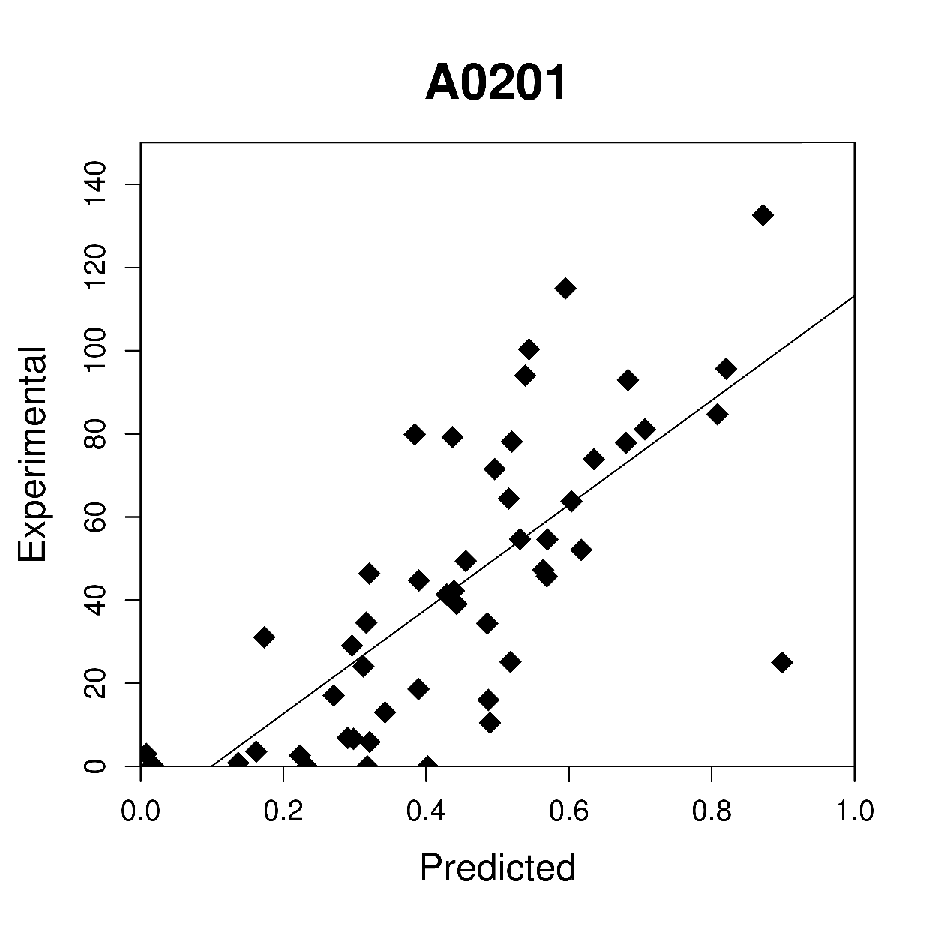
\includegraphics[width=7cm]{./Figures/chapter6/lower_res/exper_meta_1}%
\hspace{0cm}%
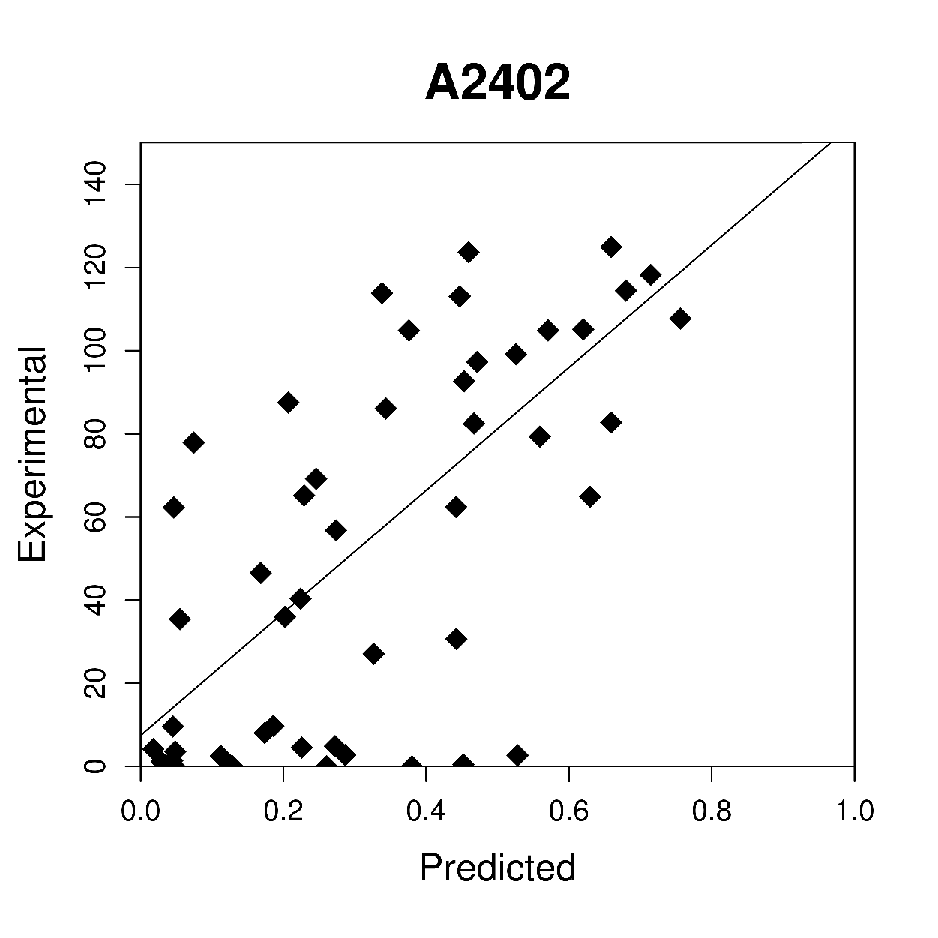
\includegraphics[width=7cm]{./Figures/chapter6/lower_res/exper_meta_2} \\
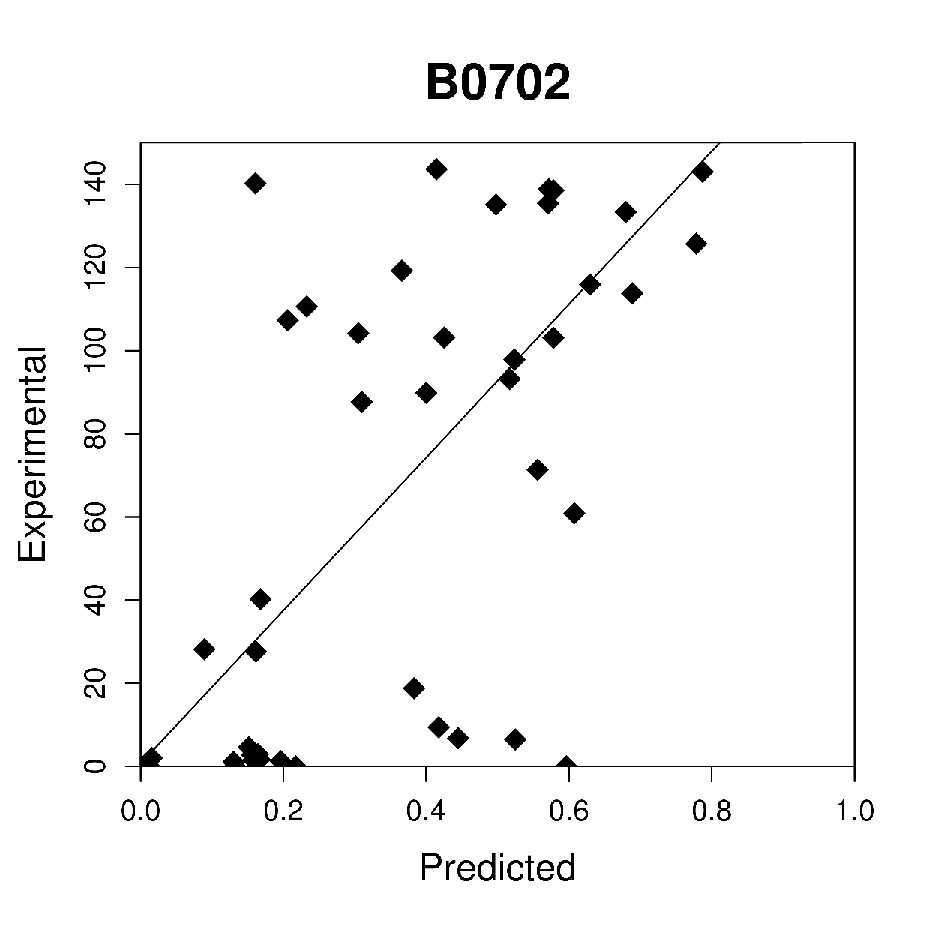
\includegraphics[width=7cm]{./Figures/chapter6/lower_res/exper_meta_3}%
\hspace{0cm}%
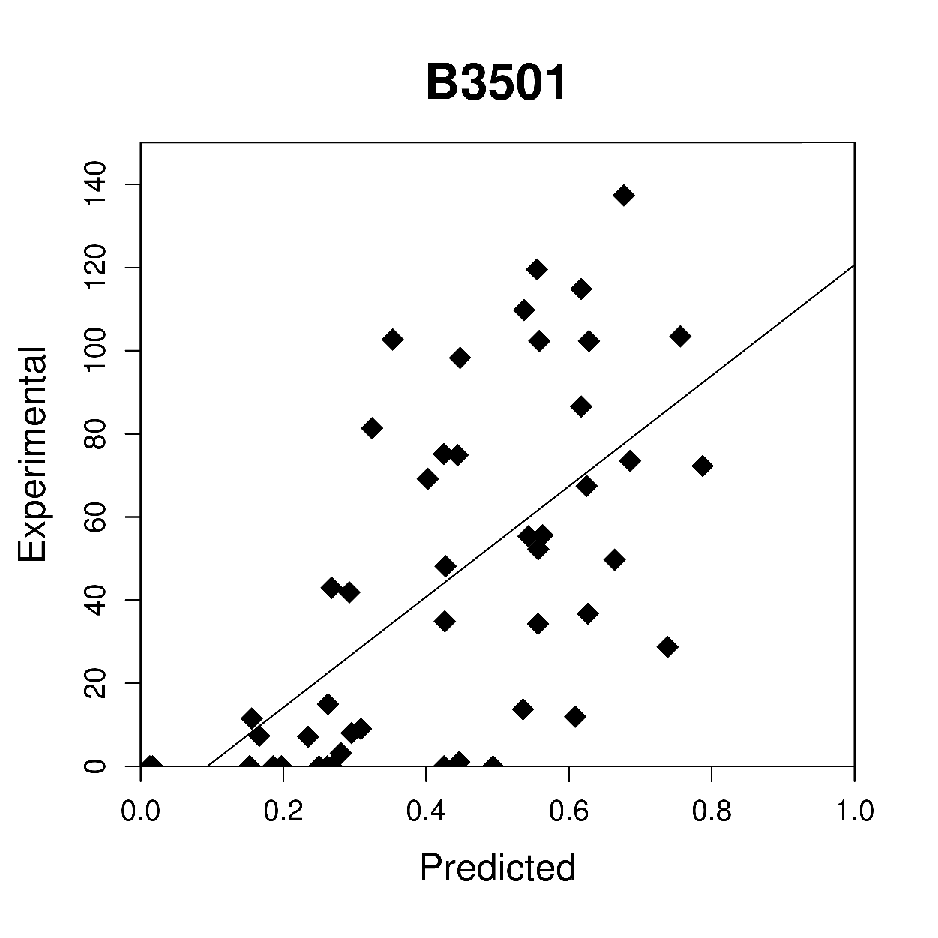
\includegraphics[width=7cm]{./Figures/chapter6/lower_res/exper_meta_4} \\
\caption[Experimental data for Metaserver]{The correlation between the experimentally measured binding affinities (\% binding compared to control peptide) and the predicted binding affinities ($1-\log _{50000} \left( \text{affinity} \right)$) of Metaserver for each of the 4 alleles analysed.}
\label{chapter6/figure1}
\end{figure}

\begin{figure}[htp]
\centering
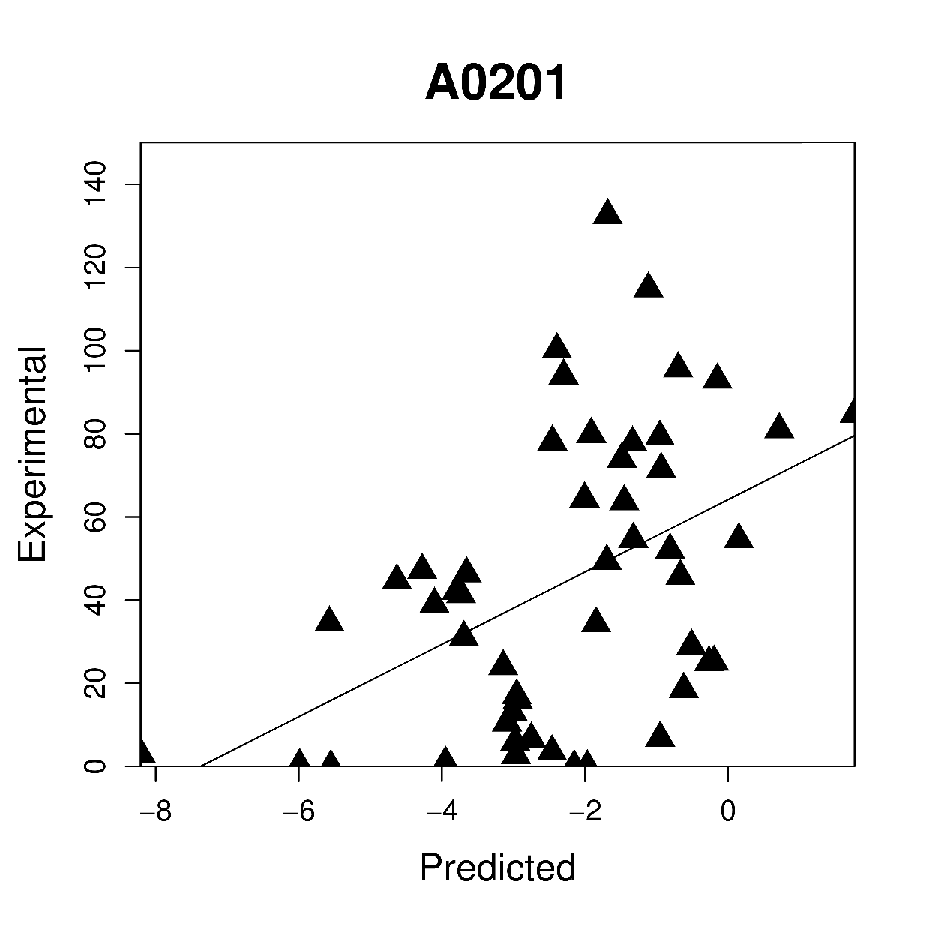
\includegraphics[width=7cm]{./Figures/chapter6/lower_res/exper_epi_1}%
\hspace{0cm}%
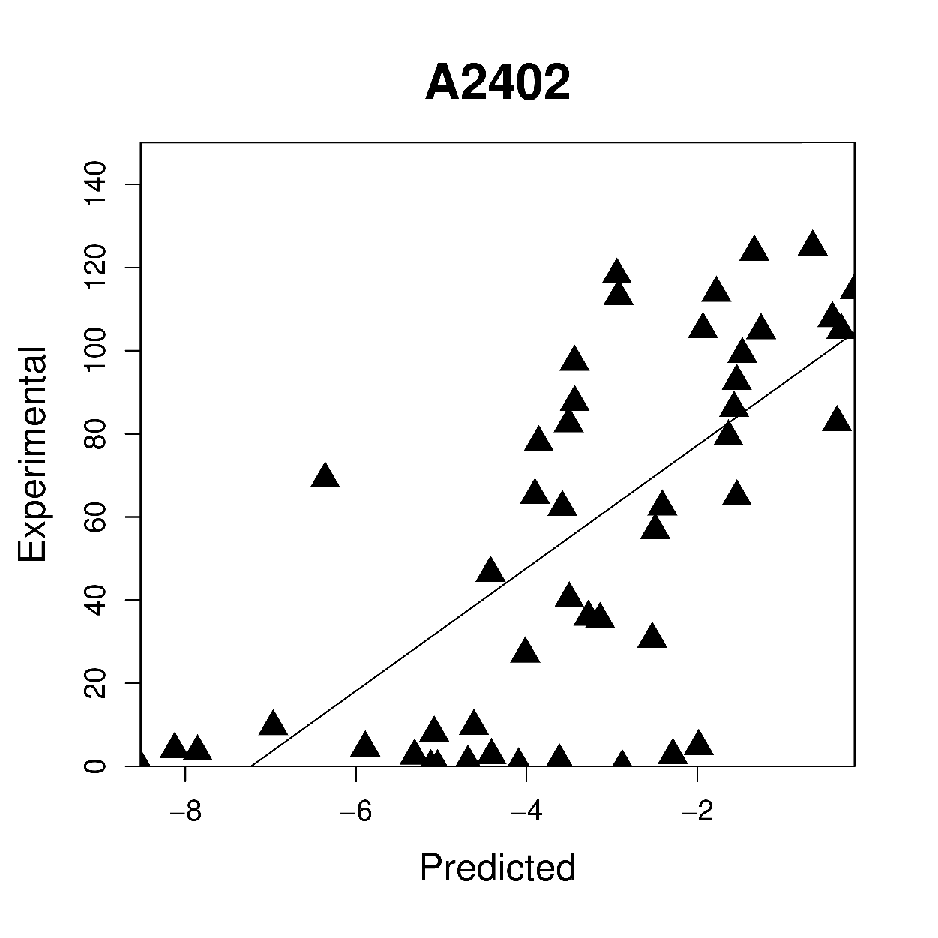
\includegraphics[width=7cm]{./Figures/chapter6/lower_res/exper_epi_2} \\
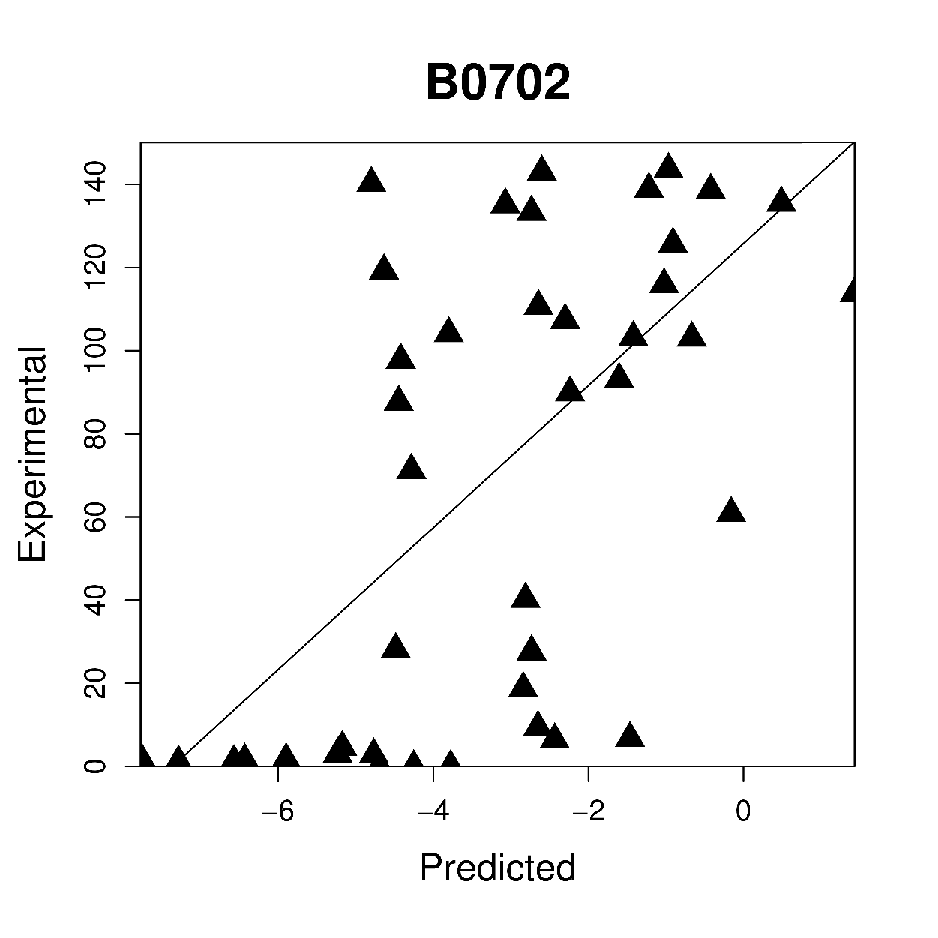
\includegraphics[width=7cm]{./Figures/chapter6/lower_res/exper_epi_3}%
\hspace{0cm}%
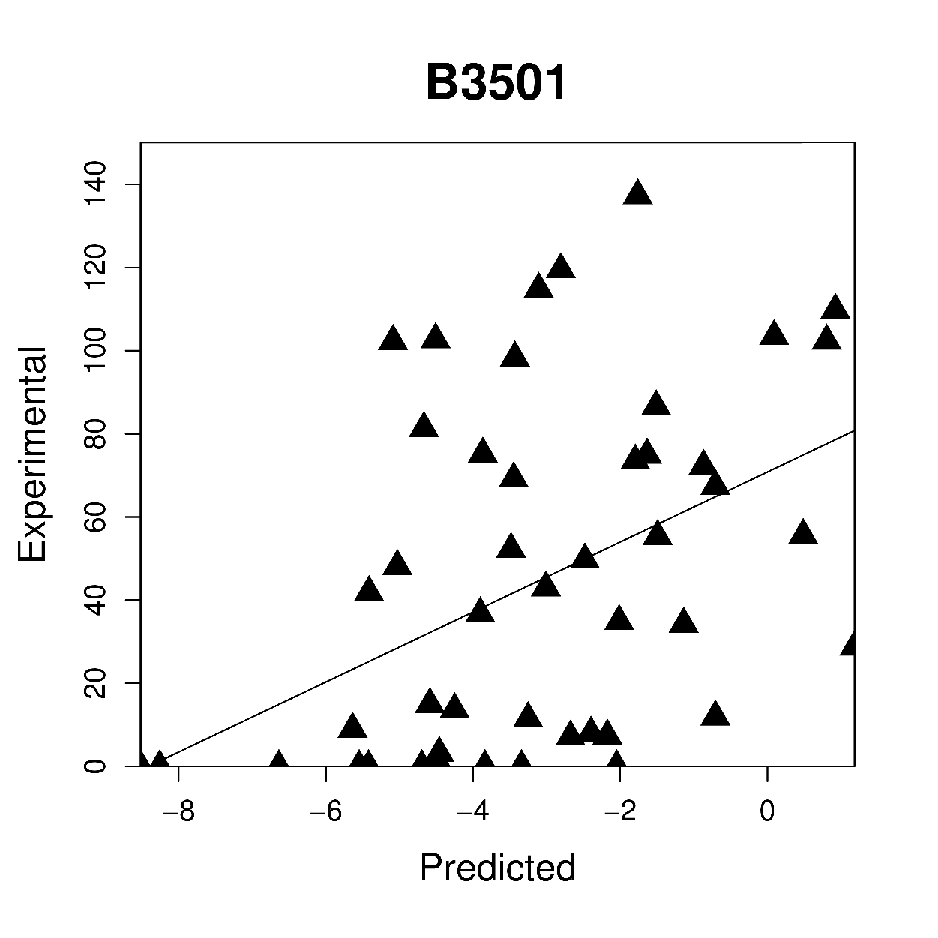
\includegraphics[width=7cm]{./Figures/chapter6/lower_res/exper_epi_4} \\
\caption[Experimental data for Epipred]{The correlation between the experimentally measured binding affinities (\% binding compared to control peptide) and the predicted binding affinities ($1-\log _{50000} \left( \text{affinity} \right)$) of Epipred for each of the 4 alleles analysed.}
\label{chapter6/figure2}
\end{figure}

\subsection{Protective class I alleles bind HBZ strongly}\label{Chapter6Result2}

A number of associations between HLA class I alleles and protection or disease risk in HTLV-I infection have been identified in a population in southern Japan \citep{Jeffery1999, Jeffery2000}. We performed a rigorous reanalysis of these associations for verification and refinement in \cref{Chapter3}. From this data, \gene{A*0201} and \gene{Cw*0801} were classed as protective alleles and \gene{B*5401} as a detrimental allele in the context of disease risk and proviral load. Hence, we started our analysis of HTLV-I epitopes with these alleles.

We compared the predicted HTLV-I peptide-binding affinities of \gene{A*0201} and \gene{Cw*0801}, with those of \gene{B*5401} (see Methods, \sref{MethodsChapter6Result2}). Peptides from the HTLV-I protein HBZ bound to HLA A*0201 and Cw*0801 significantly more strongly compared to B*5401 ($P = 0.0002$, Wilcoxon-Mann-Whitney; \fref{chapter6/figureExtra}, \tref{chapter6/tableExtra}). Repeating the analysis with another protective allele from the \gene{A*02} family, \gene{A*0206}, instead of \gene{A*0201} yielded identical conclusions ($P = 0.0007$, Wilcoxon-Mann-Whitney; data not shown). These $P$ values need to be treated with caution because the rank of the binding affinity of one HBZ peptide for A*0201 may not be independent of the rank of the binding affinity of a second peptide to A*0201 and similarly for Cw*0801 and B*5401. However, we also found that the difference in binding strength (i.e.~the rank of the top A*0201 binding peptide minus the rank of the top B*5401 binding peptide) was significantly greater for HBZ than for other HTLV-I proteins ($P < 0.001$, binomial test). This statistic is based only on the top binding peptide so it does not assume different peptides have independent binding affinity ranks. Henceforth, we only considered the top binding peptide to avoid the potential problem of dependence (see Methods, \sref{IndependenceRanks}).

\begin{figure}[htp]
\centering
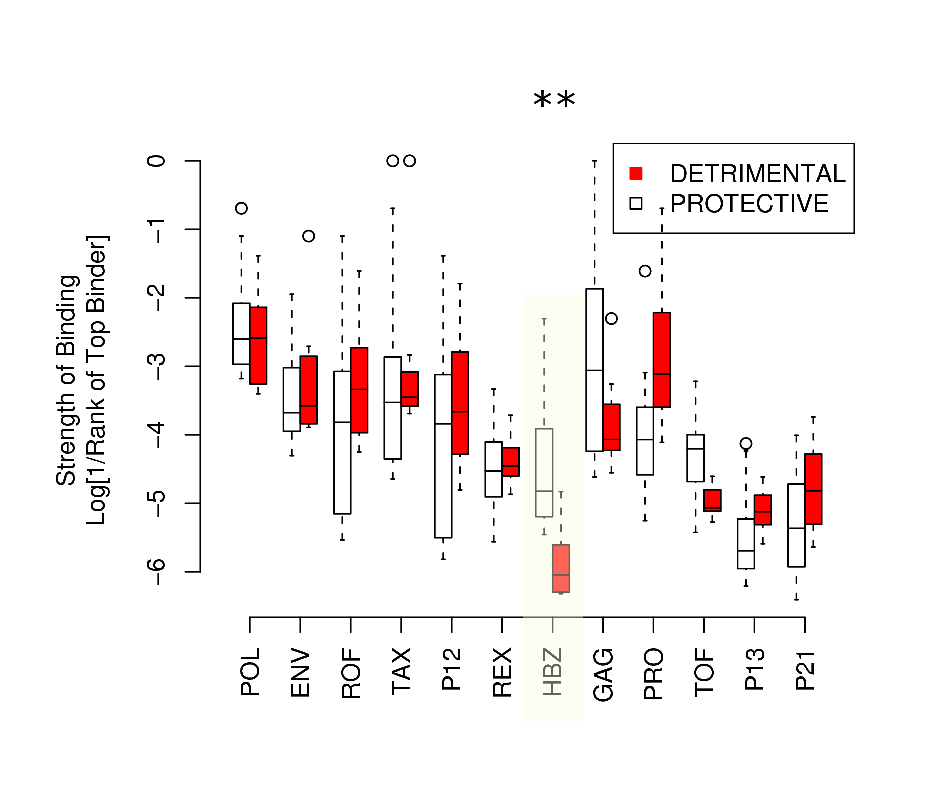
\includegraphics[width=14cm]{./Figures/chapter6/fig_2_edit}
\rule{35em}{0.5pt}
\caption[Protective class I alleles bind HBZ strongly]{The strength of binding of protective alleles (A*02/Cw*08) and detrimental alleles (B*54) across the 12 HTLV-I proteins. The y-axis gives strength of binding of the top 8 binding peptides from each protein. The level of significance indicated is corrected for multiple comparisons. All $P$ values are shown in \tref{chapter6/tableExtra}.}
\label{chapter6/figureExtra}
\end{figure}


\begin{table}[htp]
\begin{center}

\begin{tabular}{|c|c|}
\hline
Protein & Mann-Whitney 2-tailed $P$ value \bigstrut \\
\hline
Pol & 0.4999 \bigstrut[t] \\
Env & 0.5003 \\
Rof & 0.2091 \\
Tax & 0.4257 \\
P12 & 0.2978 \\
Rex & 0.5283 \\
HBZ & 0.0002 \\
Gag & 0.2572 \\
Pro & 0.0087 \\
Tof & 0.0131 \\
P13 & 0.0523 \\
P21 & 0.1200 \bigstrut[b] \\
\hline
\end{tabular}

\end{center}

\caption[Protective class I alleles bind HBZ strongly]{The $P$ values associated with \fref{chapter6/figureExtra}.}
\label{chapter6/tableExtra}
\end{table}

\subsection{Asymptomatic carriers bind HBZ more strongly than HAM/TSP patients}\label{Chapter6Result3}

Having established that the known protective HLA class I alleles bind to peptides from HBZ more strongly than the known detrimental allele, we examined peptide binding by all alleles in the Kagoshima cohort. We compared the predicted epitopes for asymptomatic carriers ($n = 202$) and HAM/TSP patients ($n = 230$) from the Kagoshima cohort. We predicted the HTLV-I peptides bound most strongly by each individual, given their HLA class I types and then tested for differences between the two subject groups (see Methods, \sref{MethodsChapter6Result3}). The results are illustrated in \fref{chapter6/figure3} and \tref{chapter6/table3}. One result remained highly statistically significant after correction for multiple comparisons and was consistent across both prediction methods: asymptomatic carriers have HLA class I alleles that bind more strongly to peptides from HBZ compared to HAM/TSP patients (Metaserver: $P = 0.0002$, Wilcoxon-Mann-Whitney. Epipred: $P < 0.0001$, Wilcoxon-Mann-Whitney; \fref{chapter6/figure3}). A bootstrap analysis was performed to confirm this result in both Metaserver and Epipred (\fref{chapter6/BootstrapMeta} and \fref{chapter6/BootstrapEpi}).

\begin{table}[htp]
\begin{center}

%\setlength{\extrarowheight}{1.5pt}
%\setlength{\tymin}{2cm}
%\tymax=\maxdimen
\begin{tabulary}{0.8\textwidth}{|l|p{1.5cm}|L|L|p{1.5cm}|L|L|}
\hline
& \multicolumn{3}{c|}{Metaserver} & \multicolumn{3}{c|}{Epipred} \\
\hline
Protein & $P$ value (2 tailed) & Group with strongest binding & Significance after correction & $P$ value (2 tailed) & Group with strongest binding	& Significance after correction \\
\hline
pol & 0.0005 & AC & ** & 0.0744 & AC & - \\
env & 0.0019 & HAM & * & 0.7203 & HAM & - \\
rof & 0.0023 & HAM & * & 0.0127 & HAM & - \\
tax & 0.3320 & AC & - & 0.8320 & HAM & - \\
p12 & 0.0168 & HAM & - & 0.0940 & HAM & - \\
rex & 0.4706 & AC & - & 0.7639 & AC & - \\
HBZ & 0.0002 & AC & ** & 0.000002 & AC & *** \\
gag & 0.0011 & AC & * & 0.1265 & HAM & - \\
pro & 0.0970 & HAM & - & 0.0143 & HAM & - \\
tof & 0.4111 & HAM & - & 0.0256 & HAM & - \\
p13 & 0.8524 & AC & - & 0.7308 & AC & - \\
p21 & 0.0341 & AC & - & 0.0018 & HAM & * \\
\hline
\end{tabulary}
\end{center}

\caption[The binding strength to all HTLV-I proteins of HAM/TSP and AC alleles]{The differences in the strength of binding of the alleles between AC and HAM/TSP patients to each of the 12 HTLV-I proteins.}
\label{chapter6/table3}
\end{table}

\begin{figure}[htp]
\centering
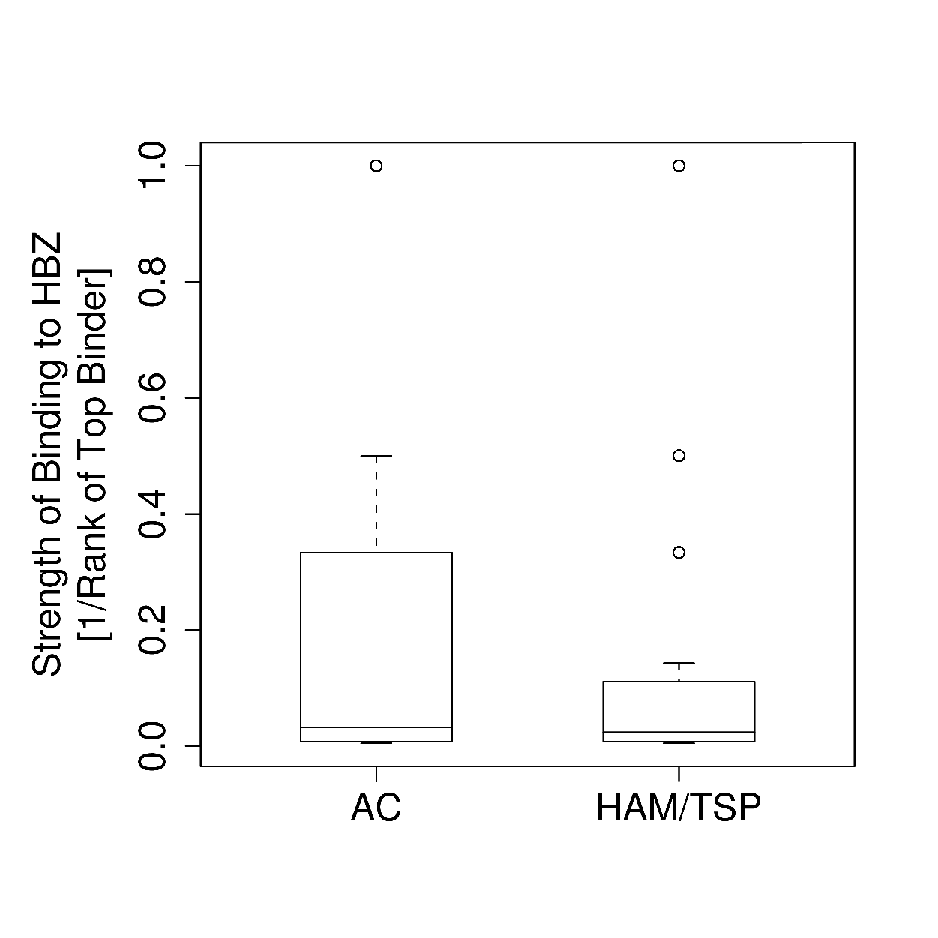
\includegraphics[width=7cm]{./Figures/chapter6/lower_res/fig_3_meta}%
\hspace{0cm}%
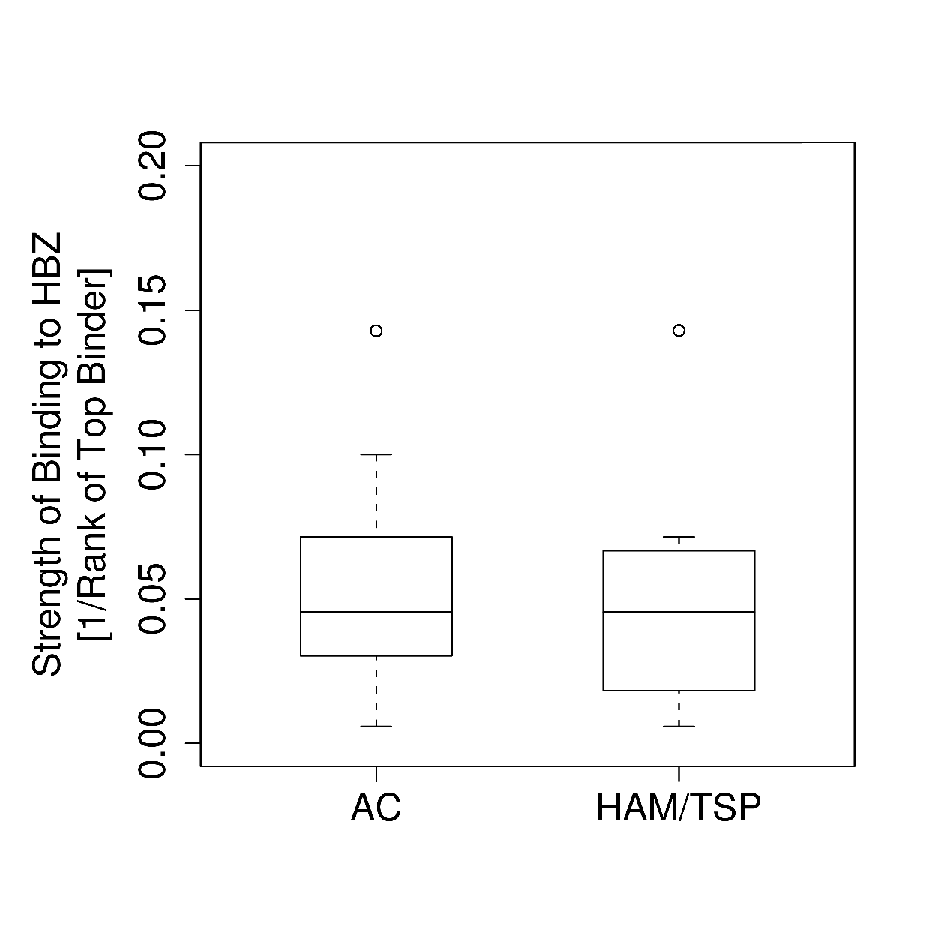
\includegraphics[width=7cm]{./Figures/chapter6/lower_res/fig_3_epi} \\
\caption[The strength of binding to HBZ]{The strength of binding of the HLA class I alleles of asymptomatic carriers and HAM/TSP patients to HBZ. Asymptomatic carriers have HLA class I alleles that bind HBZ significantly more strongly than HAM/TSP patients (Metaserver, left panel: $P = 0.0002$. Epipred, right panel: $P = 2 \times 10^{-6}$).}
\label{chapter6/figure3}
\end{figure}

To test whether this association was caused solely by the known protective and detrimental HLA alleles, the analysis for HBZ was repeated excluding A*02 and B*54. The results showed that, amongst the HLA-A alleles, A*02 was responsible for the protective effect, whereas in HLA-B more than one allele contributed significant effects. Overall, strong binding of HBZ peptides was associated with asymptomatic status, even when A*02, B*54 and Cw*08 were excluded from the analysis (Metaserver: $P = 0.04$, Wilcoxon-Mann-Whitney. Epipred: $P = 0.006$, Wilcoxon-Mann-Whitney; \tref{chapter6/table2}).

\begin{table}[htp]
\begin{center}

\newcommand{\rr}{\raggedright}
\newcommand{\tn}{\tabularnewline}

{
	\renewcommand{\arraystretch}{1.2}
	\begin{tabular}{|l|l|p{2.5cm}|p{4cm}|}
	\hline
	\multicolumn{2}{|c|}{} & \rr Whole cohort ($N=202, 230$) & \rr Excluding A*02 \& B*54 ($N=84,116$) \tn
	\hline
	\multirow{3}{*}{Metaserver} & A alleles & 0.006 & 0.81 \tn
	& B alleles & 0.001 & 0.01 \tn
	& Combined & 0.0005 & 0.04 \tn
	\hline
	\multirow{3}{*}{Epipred} & A alleles & 0.0009 & 0.72 \tn
	& B alleles & 0.0002 & 0.001 \tn
	& Combined & 0.000001 & 0.006 \tn
	\hline
	\end{tabular}
}	
	
\end{center}

\caption[The binding strength to HBZ for HAM/TSP and AC individuals]{The difference in binding strength to HBZ between HAM/TSP patients and asymptomatic carriers. The first column gives the $P$ values of the Wilcoxon-Mann-Whitney tests for the A and B loci. The second column repeats this analysis excluding individuals with either the A*02 or B*54 alleles.}
\label{chapter6/table2}
\end{table}

\begin{figure}[p]
\centering
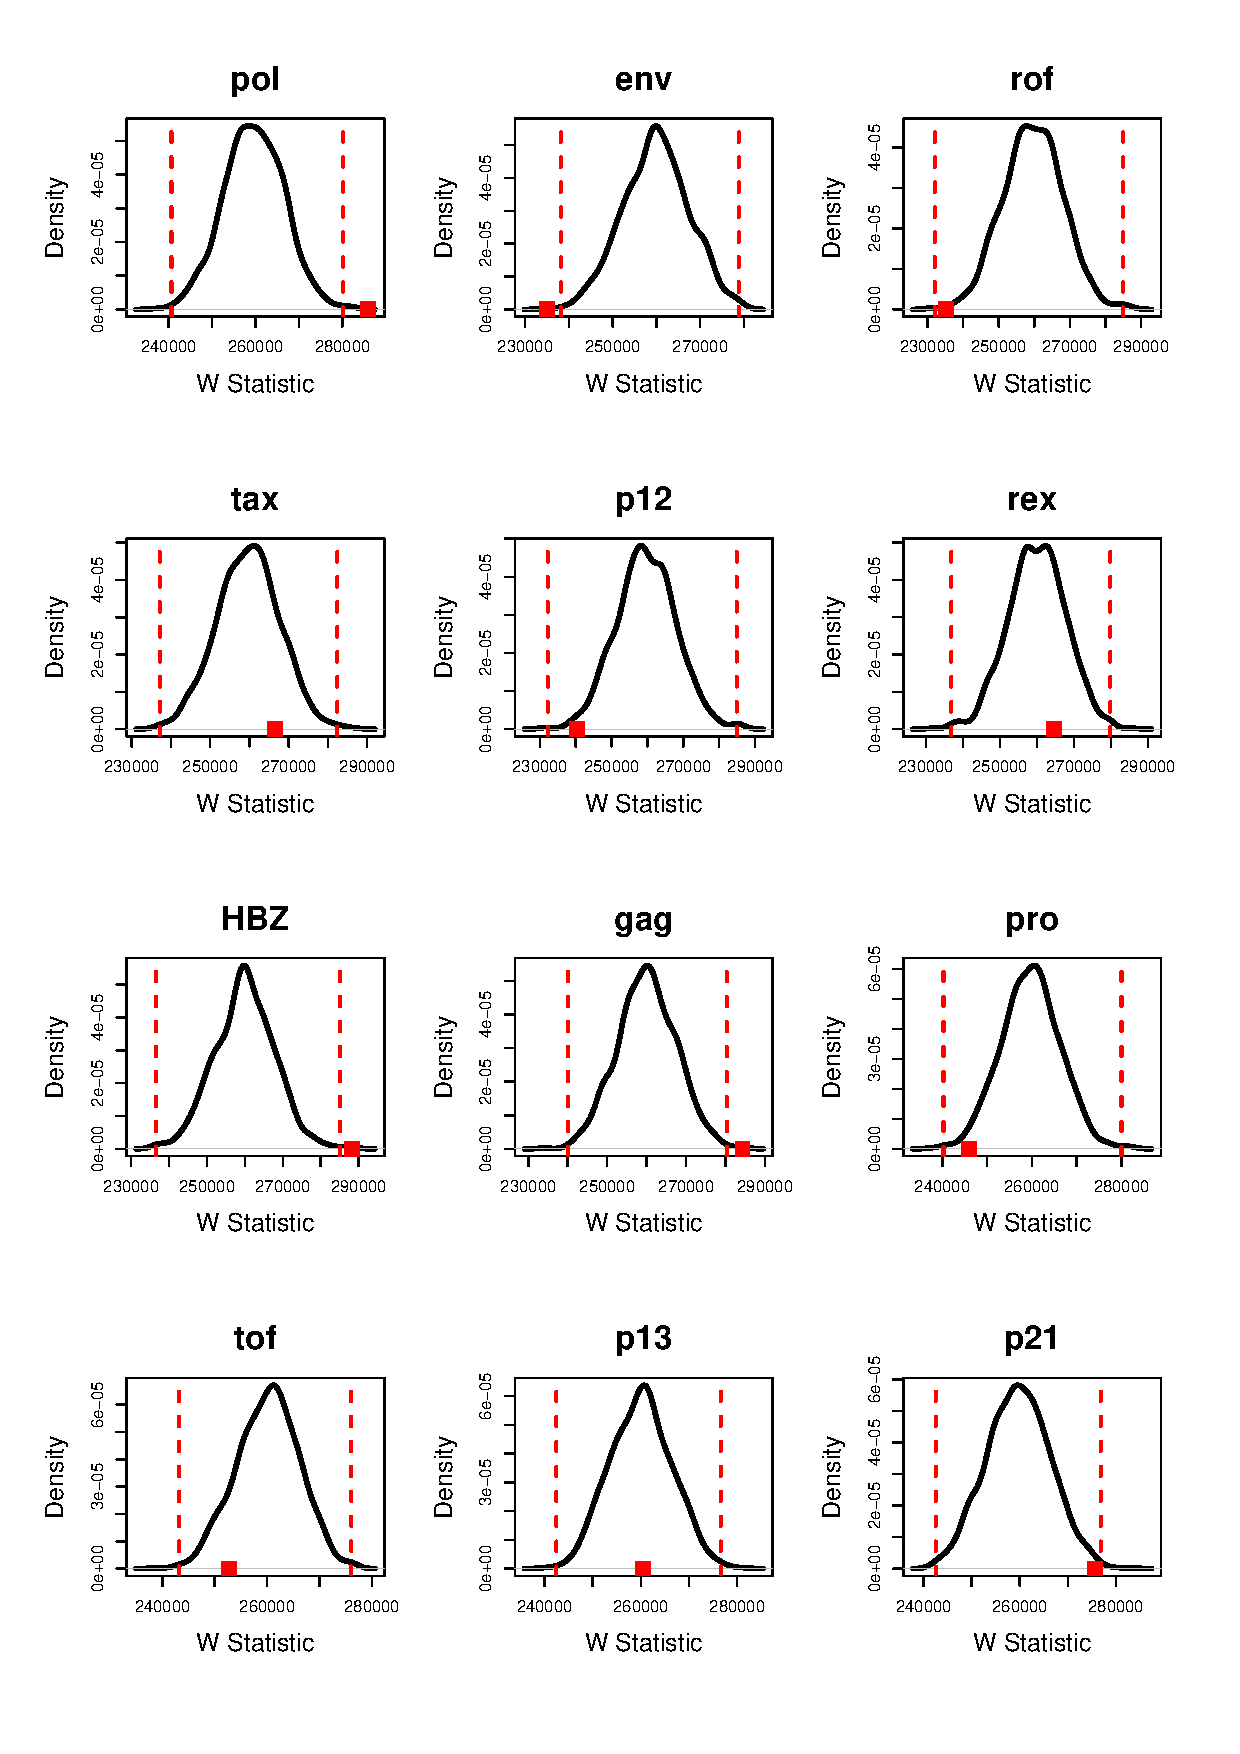
\includegraphics[width=14cm]{./Figures/chapter6/test/bootstrap_meta} \\
\caption[The bootstrap analysis for Metaserver]{A bootstrapping method to validate the conclusion of \sref{Chapter6Result3} (ACs bind HBZ more strongly than HAM/TSP patients). The 432 individuals of the Kagoshima cohort were randomly assigned to an `AC' and `HAM/TSP' group. The Mann-Whitney test was then performed on these groups. This was repeated 1,000 times and the density plot of the resultant W statistics of each test was plotted, together with the W statistic from the `true' test (red dot). The dotted lines represent the 2-tailed levels of significance after the Bonferroni adjustment for multiple comparisons. As can be seen from the HBZ graph, the W statistic value is still significantly different from the null distribution of bootstrapped W statistic values. This analysis for Metaserver was repeated for Epipred in \fref{chapter6/BootstrapEpi}.}
\label{chapter6/BootstrapMeta}
\end{figure}

\begin{figure}[p]
\centering
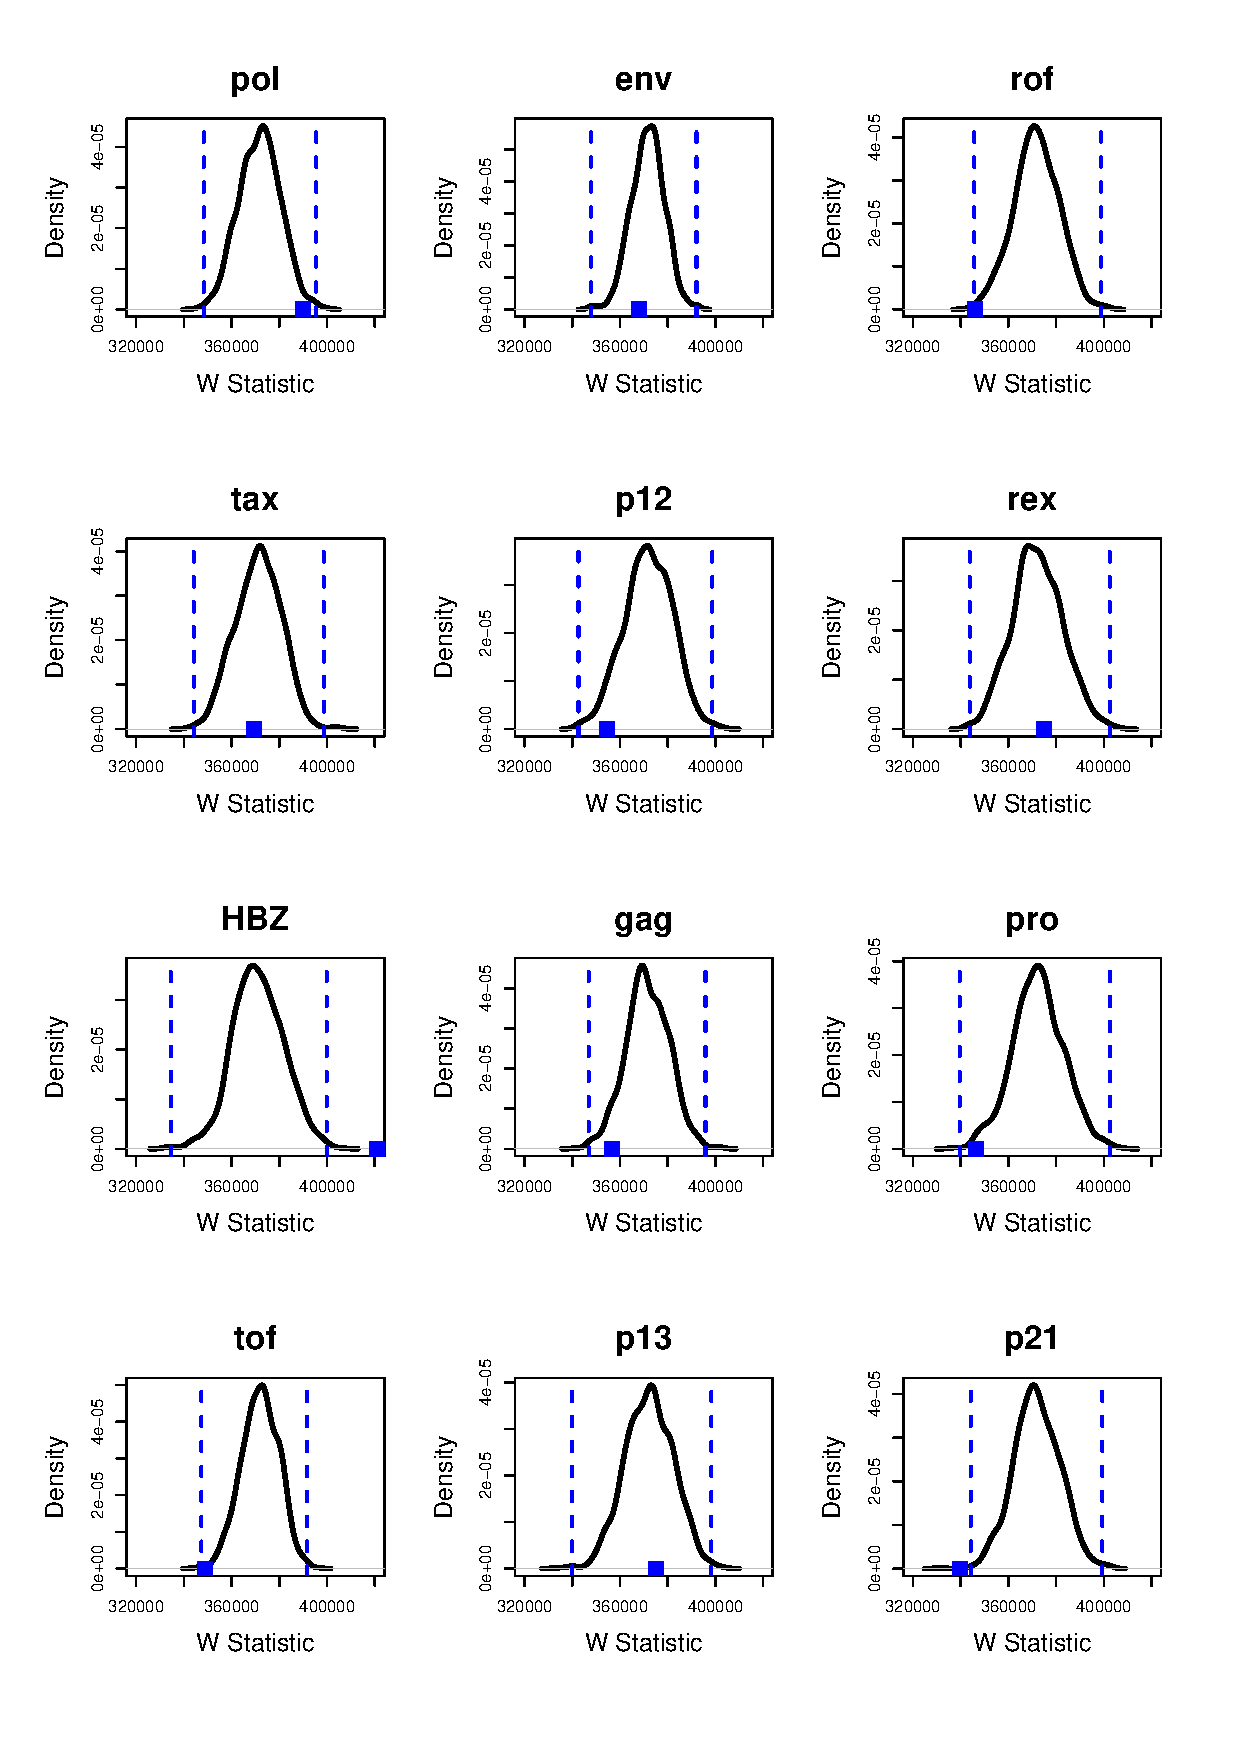
\includegraphics[width=14cm]{./Figures/chapter6/test/bootstrap_epi} \\
\caption[The bootstrap analysis for Epipred]{The bootstrap analysis for Epipred, described in \fref{chapter6/BootstrapMeta}. The W statistic value for HBZ is significantly different from the null distribution of bootstrapped W statistic values.}
\label{chapter6/BootstrapEpi}
\end{figure}

\subsection{Individuals whose HLA class I genotype predisposed them to bind HBZ peptides strongly had a significantly lower proviral load}\label{Chapter6Result4}

Next we investigated why strong binding of HBZ peptides was associated with remaining asymptomatic. One of the best predictors of HAM/TSP is a high proviral load of HTLV-I \citep{Nagai1998}. We therefore tested the hypothesis that strong predicted binding of HBZ peptides was associated with a lower proviral load. The number of alleles that each individual possessed that strongly bound peptides from HBZ was plotted against their proviral load (see Methods, \sref{MethodsChapter6Result4}). We found that the number of HLA Class I alleles that an individual had that strongly bound HBZ peptides was significantly negatively correlated with their proviral load (Metaserver: $P = 0.016$, Spearman�s rank correlation. Epipred: $P = 0.1$, Spearman�s rank correlation; \fref{chapter6/figure4}). We tested this correlation independently in HAM/TSP patients and asymptomatic carriers and then combined the $P$ values (rather than simply testing the whole cohort), so this result does not follow trivially from our previous observation than asymptomatic carriers bind HBZ significantly more strongly than HAM/TSP patients. An alternative metric, the binding strength of the top HBZ-binding peptide to each allele instead of the number of strongly binding alleles, yielded an identical conclusion i.e.~there was a significant negative correlation between the proviral load and the strength of binding to HBZ peptides (Metaserver: $P = 0.008$, Spearman�s rank correlation. Epipred: $P = 0.003$, Spearman�s rank correlation).

\begin{figure}[htp]
\centering
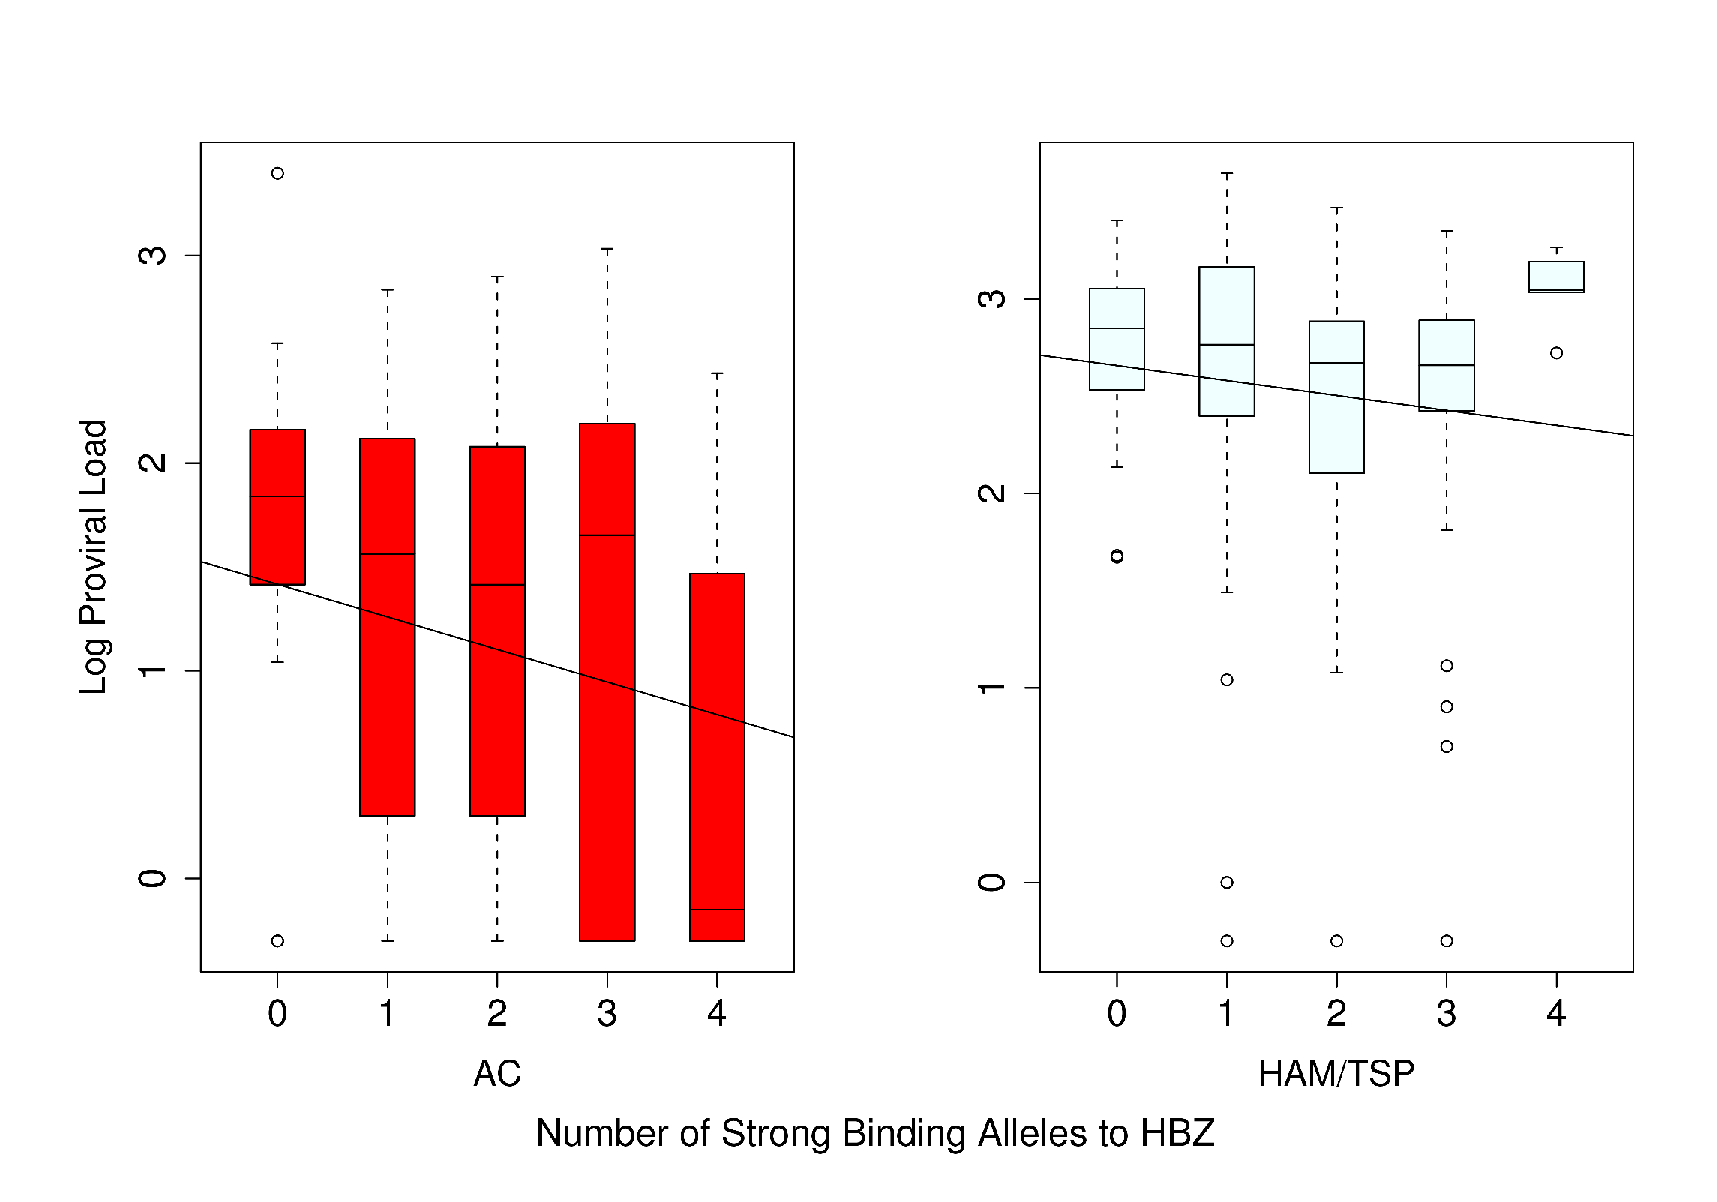
\includegraphics[width=14cm]{./Figures/chapter6/lower_res/fig_4_meta} \\
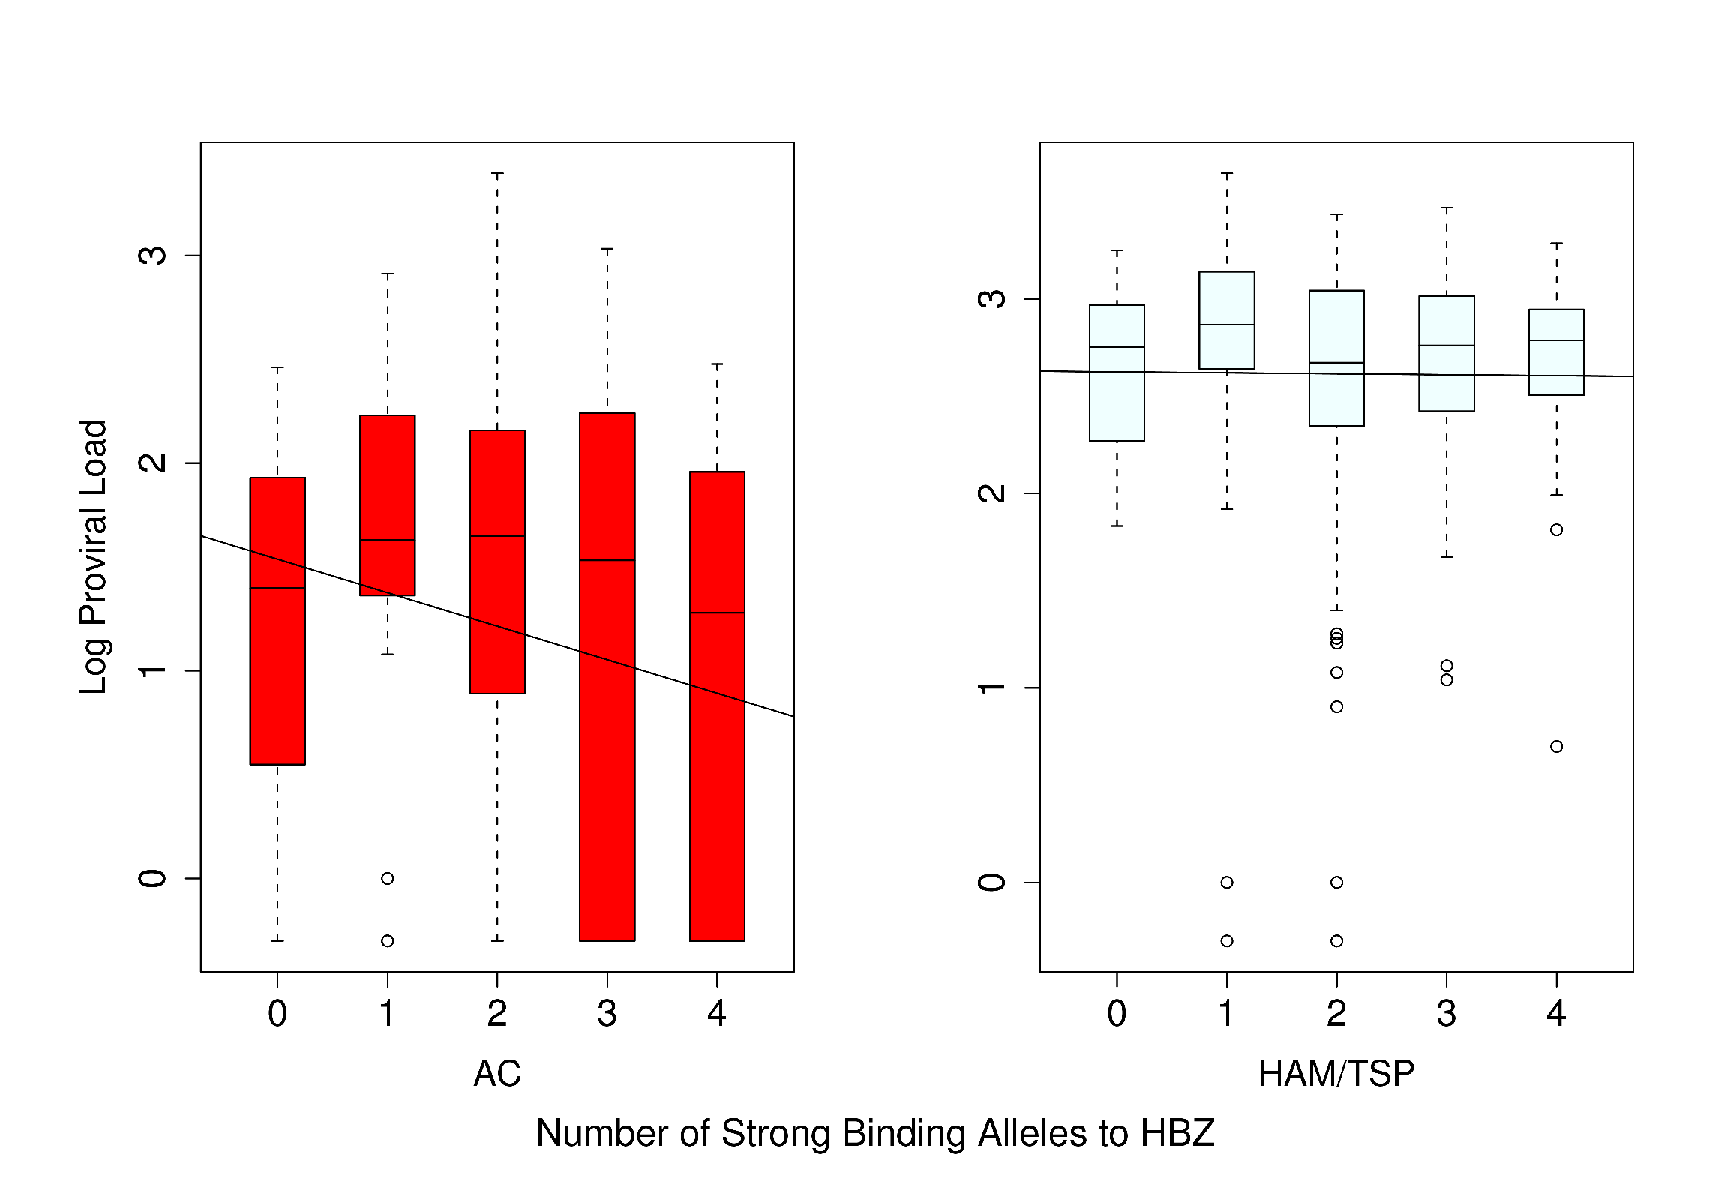
\includegraphics[width=14cm]{./Figures/chapter6/lower_res/fig_4_epi} \\
\caption[The strength of binding to HBZ and proviral load]{The count of strong binding alleles to HBZ per individual against their proviral load in AC and HAM/TSP groups. The number of strong binders to HBZ is significantly negatively correlated with proviral load (Metaserver, top panel: $P = 0.016$. Epipred, bottom panel: $0.1$).}
\label{chapter6/figure4}
\end{figure}

\subsection{HBZ Peptide Binding is a Consistent Predictor of Proviral Load}\label{chapter6/results/pred}

Next we compared our peptide-binding analysis of HLA class I genotype with a traditional frequency-based ``presence or absence of an allele'' analysis. Previously a ``traditional'' analysis yielded inconsistent results \citep{Jeffery1999, Jeffery2000, Vine2002}. For example, A*02 was a significant predictor of load in ACs but not in patients with HAM/TSP. We therefore directly compared the ability of the two methods to predict proviral load in ACs and HAM/TSP patients (\tref{chapter6/table4}). This analysis showed that whilst binding HBZ was a significant predictor of proviral load in both ACs and HAM/TSP patients ($P = 0.001$, $P = 0.017$), HLA-A*02 (presence/absence) was a significant predictor in ACs only ($P = 0.01$) and HLA-B*54 for HAM/TSP patients only ($P = 0.019$). The proportion of variance in proviral load explained was marginally higher for the peptide binding analysis. The observation that HBZ binding strength correlated with proviral load in both ACs and HAM/TSP patients suggests that peptide binding is the more fundamental predictor than HLA genotype. Further details of the predictive strength of peptide binding for proviral load and disease risk is described in \aref{AppendixC}, \sref{appendixc/log}.  

\begin{table}[htp]
\begin{center}

\begin{tabular}{|l|l|l|l|l|l|l|}
\hline
& \multicolumn{3}{c|}{Binding (A and B only)} & \multicolumn{3}{c|}{Genotype (A and B only)} \bigstrut \\
\hline
\multirow{3}{*}{AC Proviral Load} & HBZ & 0.001 & *** & \multirow{2}{*}{A*02} & \multirow{2}{*}{0.01} & \multirow{2}{*}{**} \bigstrut[t] \\
& Pro & 0.013 & * & & & \bigstrut[b] \\
\cline{2-7}
& \multicolumn{3}{c|}{$R^2 = 0.054$} & \multicolumn{3}{c|}{$R^2 = 0.034$} \bigstrut \\
\hline
\multirow{2}{*}{HAM/TSP Proviral Load} & HBZ & 0.017 & * & B*54 & 0.019 & * \bigstrut \\
\cline{2-7}
& \multicolumn{3}{c|}{$R^2 = 0.026$} & \multicolumn{3}{c|}{$R^2 = 0.025$} \bigstrut \\
\hline
\end{tabular}
\end{center}

\caption[Multiple regression models predicting proviral load]{The significant predictors and their associated P values for each of the multiple regression models of proviral load.}
\label{chapter6/table4}
\end{table}

\subsection{Proteins whose peptides are bound strongly by asymptomatic carriers are those associated with a lower proviral load}\label{chapter6/resultsProt}

In the work above we established that the HTLV-I protein that is associated with the most significant reduction in HAM/TSP risk when bound by HLA class I molecules (i.e.~HBZ, \tref{chapter6/table3}) is also, independently, associated with a significant reduction in proviral load when bound (\fref{chapter6/figure4}). We wished to investigate whether this relationship held across all proteins. We ranked each HTLV-I protein by the following criteria: 

\begin{enumerate}
\item Is strong binding of peptides from this protein associated with a lower HAM/TSP prevalence? 
\item Is strong binding of peptides from this protein associated with a lower proviral load (tested independently in AC and HAM/TSP groups and then recombined, to avoid trivial associations)?
\end{enumerate}

\tref{chapter6/table2HypothRank} illustrates this concept. The first column ranks the HTLV-I proteins according to whether they were bound more strongly by asymptomatic carriers or HAM/TSP patients (\fref{chapter6/figure5Meta} x-axis; at the extremes ACs were significantly more likely to bind peptides from HBZ, HAM/TSP patients were significantly more likely to bind peptides from Env). This list could be viewed as the ``rank order of targets for a vaccine designed to reduce HAM/TSP risk''. The second column ranks the proteins according to whether binding their peptides was associated with a lower proviral load (\fref{chapter6/figure5Meta}, y-axis; at the extremes binding of HBZ was associated with a significantly lower proviral load, binding of Env was associated with a significantly higher proviral load). This list could be viewed as the ``rank order of targets for a vaccine designed to reduce proviral load''.  

We then compared these two sets of ranks and found them to be strongly positively correlated (Metaserver: $R_S = 0.86$, $P = 0.0005$, Spearman�s rank correlation; \fref{chapter6/figure5Meta}. Epipred: $R_S = 0.66$, $P = 0.02$, Spearman�s rank correlation; \fref{chapter6/figure5Epi}). That is, proteins whose peptides are bound strongly by asymptomatic carriers are, independently, those associated with a lower load when bound. This observation has two important implications. Firstly, HLA class I binding of peptides from different proteins has a differential impact on both proviral load and HAM/TSP risk. Secondly, the fact that across all alleles and across all proteins, peptide binding associated with immune control (reduced proviral load) is strongly correlated with prevention of HAM/TSP is the strongest evidence yet that the CD8$^+$ T cell response can have a beneficial role in HTLV-I infection.

\begin{table}[htp]
\centering
\begin{tabular}{|c|c|c|}
\hline
& \multicolumn{2}{c|}{Targeting this protein is associated with:} \bigstrut \\
\hline
& Reduced HAM/TSP Frequency & Reduced Proviral Load \bigstrut \\
\hline
\multirow{3}{*}{\begin{sideways}Best\end{sideways}} & HBZ & Gag \bigstrut[t] \\
& Pol & HBZ \\
& Gag & Pol \\
\multirow{6}{*}{$\downarrow$} & P21 & Rex \\
& Tax & Tof \\
& Rex & P21 \\
& P13 & Pro \\
& Tof & Tax \\
& Pro & P13 \\
\multirow{3}{*}{\begin{sideways}Worst\end{sideways}} & P12 & P12 \\
& Rof & Rof \\
& Env & Env \bigstrut[b]\\
\hline
\end{tabular}
\caption[The rank order of HTLV-I protein targets]{The rank order of targeting HTLV-I proteins according to their potential to reduce the risk of HAM/TSP (first column) and reduce proviral load (second column).}
\label{chapter6/table2HypothRank}
\end{table}

\begin{figure}[htp]
\centering
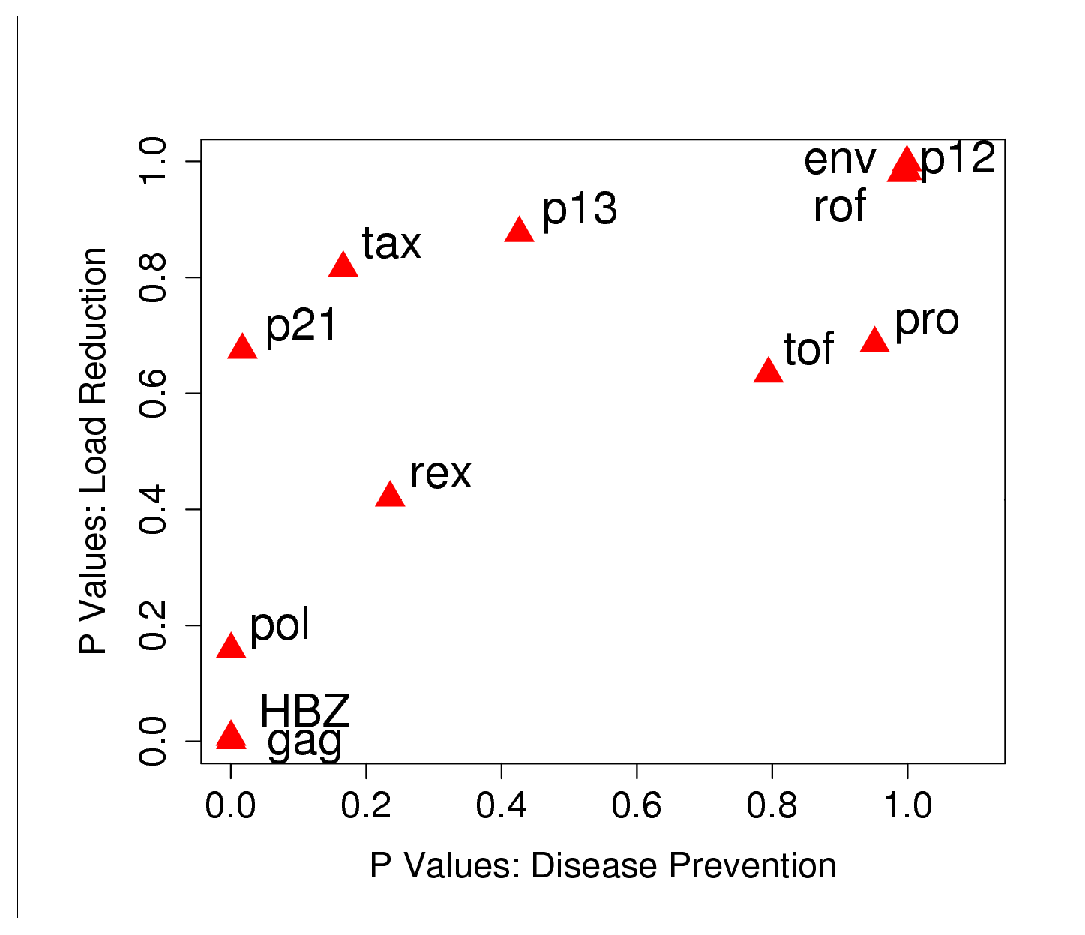
\includegraphics[width=14cm]{./Figures/chapter6/lower_res/fig_5_meta}
\rule{35em}{0.5pt}
\caption[The correlation of hypotheses for Metaserver]{The correlation between the $P$ values of the 1-tailed hypotheses: targeting this protein is associated with a lower proviral load and targeting this protein is associated with a lower HAM/TSP prevalence ($R_S=0.86$, $P = 0.0005$). In addition to HBZ, Gag also produced significant results in this analysis (it was significantly associated with a lower HAM/TSP prevalence ($P = 0.0005$) and a lower proviral load ($P = 0.002$)). However, we did not focus on this result as it was not repeated independently with Epipred.}
\label{chapter6/figure5Meta}
\end{figure}

\begin{figure}[htp]
\centering
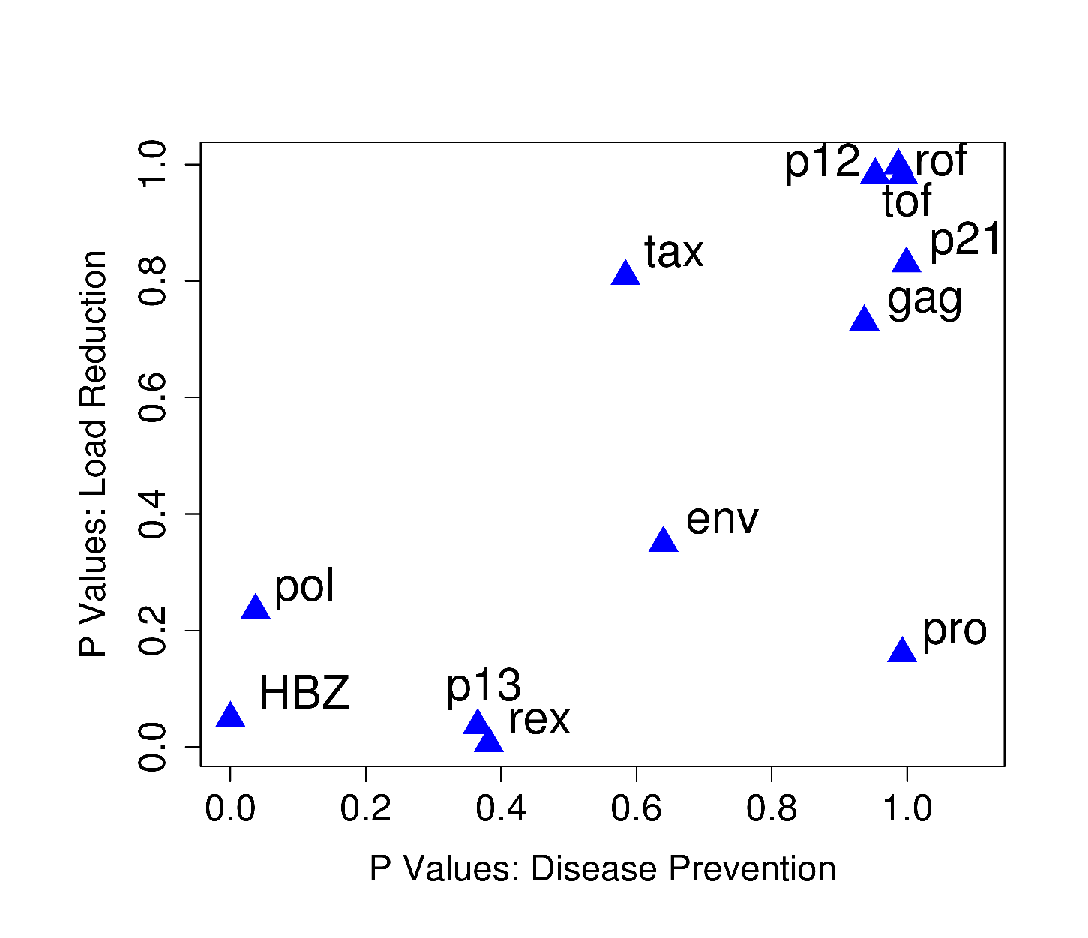
\includegraphics[width=14cm]{./Figures/chapter6/lower_res/fig_5_epi}
\rule{35em}{0.5pt}
\caption[The correlation of hypotheses for Epipred]{The correlation between the $P$ values of the 2 hypotheses: targeting this protein is associated with a reduction in HAM/TSP prevalence and targeting this protein is associated with a reduction in proviral load ($R_S=0.66$, $P = 0.02$). Epitope binding predictions made using Epipred.}
\label{chapter6/figure5Epi}
\end{figure}

\subsection{The Prevented Fraction of Disease, F\subscript{P}}\label{Chapter6ResultFP}

We calculated the prevented fraction of disease attributable to the possession of one or more strong binding alleles to HBZ \citep{Jeffery1999} (see Methods, \sref{MethodsChapter6FP}). This showed that the possession of strong HBZ-binding HLA alleles prevented $\left( F_P \right) \sim 48\% \left( SD \, 12.3\% \right)$ of potential cases of HAM/TSP in the study population. However, the strength of HBZ binding is not the only determinant of disease status: in a logistic regression model, the strength of HBZ binding alone could only predict 55\% of cases of HAM/TSP.

\subsection{HBZ Specific CD8$^+$ T Cells can be Detected \emph{ex vivo}}

This work strongly implies that HBZ-specific CD8$^+$ T cells play a protective role in HTLV-I infection. HBZ immunogenicity has been studied in ATL patients \citep{Satou2006, Matsuoka2009} but it is unknown whether a HBZ-specific CD8$^+$ T cell response is generated or even whether HBZ protein is expressed in asymptomatic carriers and HAM/TSP patients. We therefore sought to identify HBZ-specific CD8$^+$ T cells in PBMCs from HTLV-I infected individuals. We assayed IFN-$\gamma$ production by ELISpot following stimulation in vitro with a pool of overlapping peptides that spanned the entire HBZ protein. Of 45 subjects tested, 31\% had detectable HBZ-specific CD8$^+$ T cells. We conclude that HBZ protein is expressed in vivo and is immunogenic.

\subsection{The Comparative Immunogenicity of HBZ and Tax}

How does the immunogenicity of HBZ compare to Tax? We compared the predicted top binding peptide from HBZ and Tax to 43 alleles (the allele capacity of Metaserver). Peptides from Tax bind significantly more strongly than peptides from HBZ ($P = 0.00002$, paired Wilcoxon-Mann-Whitney; \fref{chapter6/figureImmun}, panel A). Consistent with this, the frequency of Tax-specific CD8$^+$ T cells by IFN-$\gamma$ ELISpot was also greater than the frequency of HBZ-specific CD8$^+$ T cells in the 45 HTLV-I infected individuals ($P = 0.000006$, paired Wilcoxon-Mann-Whitney; \fref{chapter6/figureImmun}, panel B).

\begin{figure}[htp]
\centering
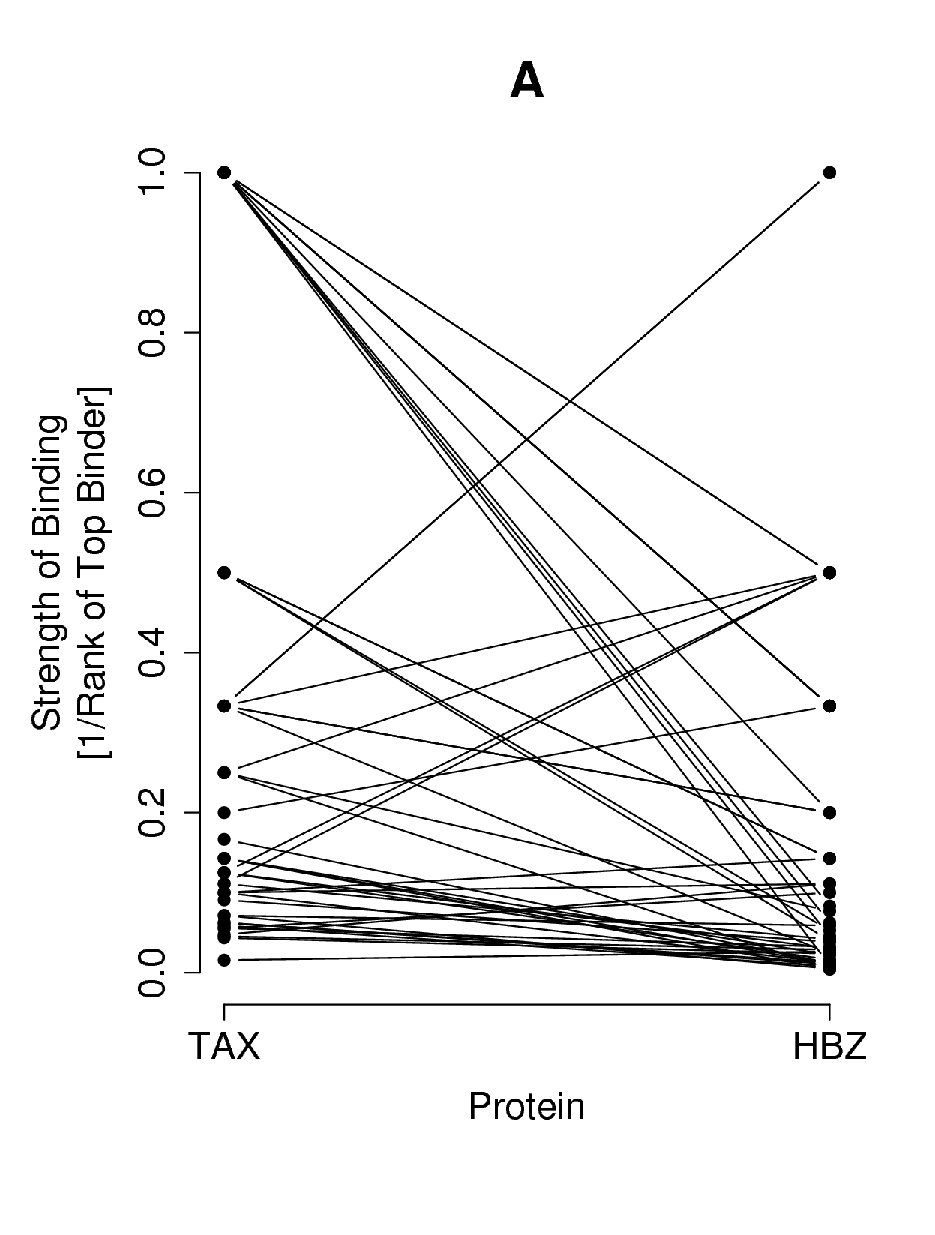
\includegraphics[width=7cm]{./Figures/chapter6/lower_res/immunogenicity_tax_hbz}%
\hspace{0cm}%
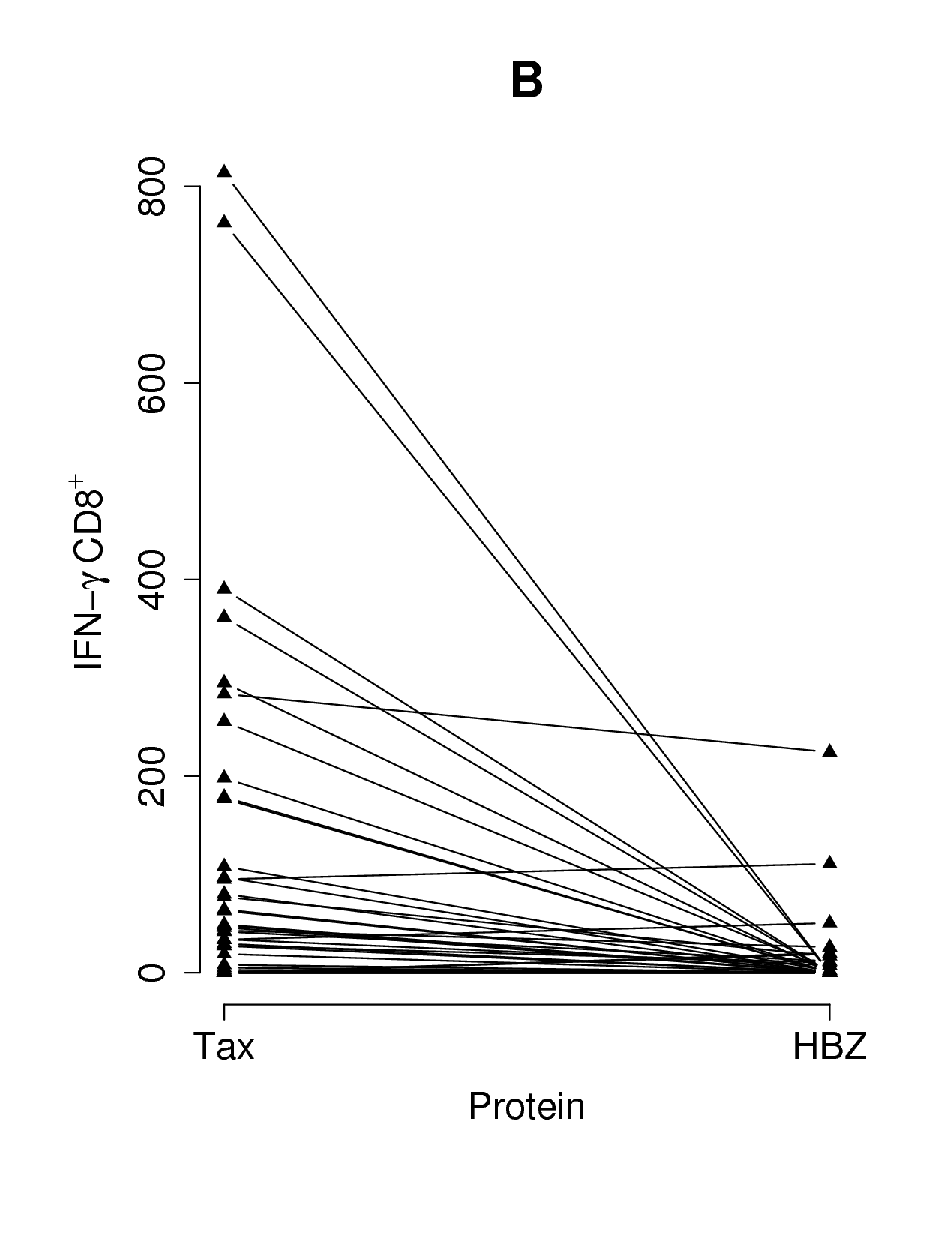
\includegraphics[width=7cm]{./Figures/chapter6/lower_res/immunogenicity_exper} \\
\caption[The comparative immunogenicity of HBZ and Tax]{The comparative immunogenicity of HBZ and Tax. A, The predicted top binding peptide from Tax and HBZ to each of the 43 alleles for which Metaserver predicts binding affinities was found. Peptides from Tax are bound more strongly than peptides from HBZ ($P = 0.00002$, paired Wilcoxon-Mann-Whitney). B, Consistent with this, the frequency of Tax-specific CD8$^+$ T cells was also greater compared to HBZ CD8$^+$ T cells in the 45 HTLV-I infected individuals tested using by IFN-$\gamma$ ELISpot ($P = 0.000006$, paired Wilcoxon-Mann-Whitney).}
\label{chapter6/figureImmun}
\end{figure}


%%%%%%%%%%%%%%%%%%%%%%%%%%%%%%%%%%%%%%%%%%%%%%%%%%%%%%%%%%%%%%%%%%%%%%%%%%%%%%%%%%%%%%%%%%%%%%%%%%%%

\begin{table}[htp]
\begin{center}

\begin{sideways}
{
\renewcommand{\arraystretch}{1.5}
\begin{tabulary}{1.5\textwidth}{|c|L|c|c|c|c|L|}
\hline
& \multirow{2}{*}{Null hypothesis} & \multicolumn{2}{c}{Rank measure} & \multicolumn{2}{|c|}{Raw score} & \multirow{2}{*}{Conclusion} \\
\cline{3-6}
& & Metaserver & Epipred & Metaserver & Epipred & \\	
\hline
1 & Protective and detrimental alleles target HBZ equally & \multicolumn{2}{c|}{$0.0002$} & - & - & Protective alleles bind HBZ significantly more strongly than detrimental alleles \\
\hline
2 & AC and HAM/TSP patients target HBZ equally & $0.0002$ & $0.000002$ & $0.002$ & $0.001$ & ACs have HLA alleles that bind HBZ significantly more strongly compared to HAM/TSP patients \\
\hline
3 & AC and HAM/TSP patients target HBZ equally (excluding A02, B54 and Cw08) & $0.04$ & $0.006$ & $0.14$ & $0.03$ & ACs bind HBZ significantly more strongly compared to HAM/TSP patients even when known protective and detrimental alleles are excluded \\
\hline
4 & There is no correlation between proviral load and the number of alleles that bind HBZ strongly & $0.016$ & $0.1$ & $0.01$ & $0.032$ & The higher the number of strong binding alleles to HBZ per individual, the lower their proviral load \\
\hline
5 & There is no correlation between proviral load and the strength of HBZ binding & $0.008$ & $0.04$ & $0.003$ & $0.085$ & The greater the strength of HBZ binding (rank method), the lower the proviral load \\
\hline
6 & There is no correlation between load reduction (count) and disease prevalence reduction & $0.0005$ & $0.02$ & $0.004$ & $0.03$ & Proteins that are strongly bound by asymptomatic carriers are, independently, those associated with a greater reduction in load when bound \\
\hline
7 & There is no correlation between load reduction (rank) and disease prevalence reduction & $< 2.2 \times 10^{-16}$ & $0.003$ & $0.002$ & $0.2$ & As above, using the rank measure to quantify the effect of binding strength on proviral load \\
\hline
\end{tabulary}
}
\end{sideways}
\end{center}

\caption[The summary of epitope prediction hypothesis testing]{The results of hypothesis testing repeated using different epitope prediction methods (Metaserver and Epipred) and different metrics (a rank measure which only compares within alleles (i.e. not between alleles) and a raw binding score measure which compares between as well as within alleles).}
\label{chapter6/table5}
\end{table}


%%%%%%%%%%%%%%%%%%%%%%%%%%%%%%%%%%%%%%%%%%%%%%%%%%%%%%%%%%%%%%%%%%%%%%%%%%%%%%%%%%%%%%%%%%%%%%%%%%%%
%%%%%%%%%%%%%%%%%%%%%%%%%%%%%%%%%%%%%%%%%%%%%%%%%%%%%%%%%%%%%%%%%%%%%%%%%%%%%%%%%%%%%%%%%%%%%%%%%%%%


\section{Discussion}\label{chapter6/discussion}

Using validated epitope prediction software, we show that strong binding of peptides from the HTLV-I basic leucine zipper factor (HBZ) protein is associated with a reduced risk of HAM/TSP and a reduced proviral load in a population with endemic HTLV-I infection in southern Japan. We demonstrated that protection is not limited to a small subset of HLA class I alleles previously associated with disease status and proviral load (HLA-A*02 and HLA-Cw*08), but is more generally associated with HLA class I alleles that bind strongly to HBZ.

Prior to this analysis CD8$^+$ T cells specific for the HTLV-I protein Tax were often considered as the best candidate for `efficient' or `protective' CD8$^+$ cells because of the immunodominance of Tax in the CD8$^+$ T cell response \citep{Kannagi1991, Goon2004}. Our finding that binding of HBZ peptides rather than Tax peptides is protective raises the question why HBZ? 

The HBZ gene was identified recently \citep{Gaudray2002}. It is encoded by the complementary strand of the HTLV-I genome and its promoter lies in the 3� LTR rather than the 5� LTR. It functions by binding to the transcription factor CREB-2. There are two major splice variants of the HBZ transcript, SP1 and SP2; the variant SP1 is more abundant and is the variant used in this study \citep{Cavanagh2006}. Expression of HBZ suppresses Tax-mediated transactivation through the 5� LTR \citep{Gaudray2002, Basbous2003} and thereby inhibits expression of other HTLV-I genes \citep{Gaudray2002, Li2009}; HBZ can be expressed in the absence of transcription of other HTLV-I genes. Additionally, HBZ RNA promotes the proliferation of infected T-lymphocytes \citep{Satou2006}. This dual action - reduction of HTLV-I expression and subsequent protection from immune surveillance, and enhancement of infected cell proliferation - probably confers a survival advantage on HBZ-expressing cells and is consistent with the observations that HBZ enhances persistence in HTLV-I inoculated rabbits \citep{Li2009} and that ATL cells often have a hypermethylated or deleted 5� LTR but an intact functional 3� LTR \citep{Satou2006}.

We hypothesise that if HBZ-specific CD8$^+$ T cells are weak or absent then infected cells that express HBZ but not other viral proteins will escape immune surveillance and proliferate rapidly, leading to a large increase in proviral load. HBZ-specific CD8$^+$ T cells would then play an important role in preventing this proliferation of provirus-positive cells and blocking this strategy of persistence. If this conclusion is correct that HLA class I recognition of HBZ plays a central role in the control of HTLV-I replication than one might expect that HBZ in HTLV-I would have evolved to minimize the effect of this class I recognition. Consistent with this hypothesis, we find that the predicted binding affinity to HBZ peptides is significantly weaker than that of Tax peptides and that the frequency of HBZ-specific CD8$^+$ T cells is significantly lower than the frequency of Tax-specific CD8$^+$ T cells. Although the low immunogenicity of HBZ is precisely what we predict given its central importance in maintaining HTLV-I persistence it is nevertheless striking that these low frequency responses are so important. This result challenges the prevailing assumption in HTLV-I research and in immunology in general that the immunodominant responses are the most interesting and important.

This approach to studying the association between HLA class I genotype and the outcome of infection has a number of strengths compared with a traditional frequency-based analysis. Firstly, it is more mechanistic: knowing that binding HBZ is associated with a reduced proviral load and disease risk compared with knowing that A*02 is associated with these outcomes is a simultaneously more fundamental and more applicable level of understanding. Secondly, identification of protective epitopes immediately suggests a practical approach to increase the efficiency of an individual�s anti-viral response. Thirdly, because the same effect (e.g.~HBZ binding) can be identified for many alleles it is less likely to be a spurious result of linkage disequilibrium or genetic stratification. Finally, effects due to multiple low-frequency alleles can be captured because analysis is made at the level of peptide binding rather than allelic frequency. 

In summary, using a novel and generalizable approach, we have identified one of the constituents of an effective CD8$^+$ T cell response in HTLV-I infection.

%%%%%%%%%%%%%%%%%%%%%%%%%%%%%%%%%%%%%%%%%%%%%%%%%%%%%%%%%%%%%%%%%%%%%%%%%%%%%%%%%%%%%%%%%%%%%%%%%%%%
%%%%%%%%%%%%%%%%%%%%%%%%%%%%%%%%%%%%%%%%%%%%%%%%%%%%%%%%%%%%%%%%%%%%%%%%%%%%%%%%%%%%%%%%%%%%%%%%%%%%